\documentclass[12pt, a4paper, twoside, openright]{report}
\usepackage[ansinew]{inputenc}
\usepackage[T1]{fontenc}
\usepackage[ngerman]{babel}
\usepackage{graphicx}
\usepackage{fancyhdr}
\usepackage{array}
\usepackage{bibgerm}
\usepackage{listings}
\usepackage{color}
\usepackage{setspace} 						% zeilenabstand
\usepackage{parskip}							% absatzabstand
\usepackage{titling}

% 1,5 zeilenabstand
\onehalfspacing

% pfad, wo nach bilder gesucht werden soll
\graphicspath{{images/}}

% neuer spaltentyp der wie p spalten in gr��e aufteilt aber gleichzeitig zentriert
\newcolumntype{P}[1]{>{\centering\arraybackslash}p{#1}}

%%%%%%%%%%%%%%%%%%%%%%%%%%%%%%%%%%%%%%%%%%%%%%%%%%%%%%%
%%%%%%%%%%%%%%%% fancy header and footer %%%%%%%%%%%%%%
%%%%%%%%%%%%%%%%%%%%%%%%%%%%%%%%%%%%%%%%%%%%%%%%%%%%%%%

\fancyfoot{}
\fancyfoot[RO, LE]{\thepage}
\fancyhead{}
\fancyhead[RO, LE]{\rightmark}
\fancyhead[LO, RE]{\ifnum\thechapter > 0 \leftmark \fi}
\fancypagestyle{plain}{%
\fancyhf{} % clear all header and footer fields
\fancyfoot{}
\fancyhead{}
\fancyfoot[RO, LE]{\thepage}
\renewcommand{\headrulewidth}{0pt}}
	
%%%%%%%%%%%%%%%%%%%%%%%%%%%%%%%%%%%%%%%%%%%%%%%%%%%%%%%
%%%%%%%%%%%%%%%% define colors %%%%%%%%%%%%%%%%%%%%%%%%
%%%%%%%%%%%%%%%%%%%%%%%%%%%%%%%%%%%%%%%%%%%%%%%%%%%%%%%

\definecolor{darkgreen}{rgb}{0,0.6,0}
\definecolor{gray}{rgb}{0.5,0.5,0.5}
\definecolor{purple}{rgb}{0.58,0,0.82}

%%%%%%%%%%%%%%%%%%%%%%%%%%%%%%%%%%%%%%%%%%%%%%%%%%%%%%%
%%%%%%%%%%%%%%%% listings einstellungen %%%%%%%%%%%%%%%
%%%%%%%%%%%%%%%%%%%%%%%%%%%%%%%%%%%%%%%%%%%%%%%%%%%%%%%

\lstset{frame=tb,
  language=Python,
  aboveskip=3mm,
  belowskip=3mm,
  showstringspaces=false,
  columns=flexible,
  basicstyle={\small\ttfamily},
  numbers=none,
  numberstyle=\tiny\color{gray},
  keywordstyle=\color{blue},
  commentstyle=\color{darkgreen},
  stringstyle=\color{purple},
  breaklines=true,
  breakatwhitespace=true,
  tabsize=4
}

% JavaScript erh�lt ein Markup
\lstdefinelanguage{JavaScript}{
keywords={typeof, new, true, false, catch, function, return, null, catch, switch, var, if, in, while, do, else, case, break},
keywordstyle=\color{blue}\bfseries,
ndkeywords={class, export, boolean, throw, implements, import, this},
ndkeywordstyle=\color{darkgray}\bfseries,
identifierstyle=\color{black},
sensitive=false,
comment=[l]{//},
morecomment=[s]{/*}{*/},
commentstyle=\color{gray}\ttfamily,
stringstyle=\color{purple}\ttfamily,
morestring=[b]',
morestring=[b]"
}

%%%%%%%%%%%%%%%%%%%%%%%%%%%%%%%%%%%%%%%%%%%%%%%%%%%%%%%
%%%% damit leere seiten, die vor chapters entstehen, %%
%%%% unbeschriftet sind %%%%%%%%%%%%%%%%%%%%%%%%%%%%%%%
%%%%%%%%%%%%%%%%%%%%%%%%%%%%%%%%%%%%%%%%%%%%%%%%%%%%%%%

\makeatletter
\def\cleardoublepage{\clearpage\if@twoside \ifodd\c@page\else
\hbox{}
\thispagestyle{empty}
\newpage
\if@twocolumn\hbox{}\newpage\fi\fi\fi}
\makeatother

%%%%%%%%%%%%%%%%%%%%%%%%%%%%%%%%%%%%%%%%%%%%%%%%%%%%%%%
%%%%%%%%%%%%%%%%%%%% sonstiges %%%%%%%%%%%%%%%%%%%%%%%%
%%%%%%%%%%%%%%%%%%%%%%%%%%%%%%%%%%%%%%%%%%%%%%%%%%%%%%%

\title{Untersuchung der Distributed Ledger Technologien auf Zukunftstauglichkeit}
\author{Janusz Spatz and Jens Altrock}
\date{\today}



\begin{document}

\begin{titlepage}
	\begin{center}
		
\includegraphics[scale=0.85]{hsblogo.png}
		
		\hrulefill
		
		\Large
		\textbf{Bachelor-Thesis}\\
		
		\vspace{0.5cm}
		\normalsize
		zur Erlangung des akademischen Grades\\
		Bachelor of Science (B.Sc.)\\
		
		\vspace{1cm}
		
		\LARGE
		\textbf{\thetitle}
		
		\hrulefill
		
		\vspace{0.5cm}
		\normalsize
		Fakult�t 4 - Elektrotechnik und Informatik
		
		\begin{tabular}{ll}
		Erstpr�fer: & Lars Braubach\\
		Zweitpr�fer: & Martin Hering-Bertram\\
		Abgabetermin: & 15.10.2018
		\end{tabular}
		
		\vspace{1,5cm}
		
		vorgelegt von
		
		\begin{tabular}{cc}
		Jens Altrock & Janusz Spatz\\
		399421 & 399341
		\end{tabular}
		
	\end{center}
\end{titlepage}
\cleardoublepage
\pagenumbering{gobble}
\cleardoublepage
\pagestyle{fancy}
\pagenumbering{roman}

\tableofcontents
\listoffigures
\listoftables

\cleardoublepage
\pagenumbering{arabic}

\chapter{Einleitung}
Seit 2017 besteht ein starker Wachstum des Interesses an Blockchain, wobei Bitcoin als prominenteste Implementation angesehen wird.(QUELLE) Am Sonntag, den 17. Dezember 2017 durchbricht Bitcoin erstmals fast die \$20.000 Marke (\$19,783.21)~\cite{ja:bitcoin20000}(FOOTNOTE). Doch nicht nur Bitcoin hat von dem starken Interesse profitiert, sondern auch viele weitere Kryptow�hrungen sowie andere Blockchain-Implementierungen. Damit war die Technologie in das Bewusstsein der breiten Masse gerutscht und zugleich h�ufen sich Fragen im Bezug auf Zukunftssicherheit und Tauglichkeit der jeweiligen Technologien. Jene Fragen sollen in dieser Bachelorarbeit er�rtert werden.

\section{Kooperationen mit Blockchain/Tangle}
Immer mehr kommerzielle Firmen entdecken das Potenzial von Kryptow�hrungen und weiteren Blockchain-Technologien.(QUELLE) Die Kooperation zwischen dem Automobilhersteller VW und diversen Kryptow�hrungen ist ein aktuelles Beispiel in dem eine Firma Potential in dieser Technologie sieht.
In einer am 8. August, 2018 ver�ffentlichten Kurznachricht auf der Social-Media-Plattform Twitter schreibt die Volkswagen Group:

\begin{quote}
"`Bringing \#blockchain systems to the road: We�re working full steam ahead on making super-safe \#cryptosystems available to our customers. For filling the tank, unlocking your car � and all kinds of other possibilities: \#bitcoin \#ethereum \#iota"'

- Volkswagen Group auf Twitter\footnote{https://twitter.com/VWGroup/status/1027205629436407810}
\end{quote}

In einem Blockeintrag der Volkswagen Group geht hervor, dass sie anhand von Blockchains, die Zuverl�ssigkeit und Sicherheit von Autos erh�hen wollen. Zum Beispiel indem Kilometerz�hler vor Manipulationen gesch�tzt und Hackerangriffe auf selbstfahrende Autos vorgebeugt werden.[2](QUELLE)

Auch weitere Firmen wie Bosch geben in einer Pressemitteilung Ende 2017 bekannt, dass auch sie in IOTA investieren und eng mit ihnen an verschiedenen Fronten zusammenarbeiten werden. [3](QUELLE) Sowie auch Microsoft hat sich die Kryptow�hrungen zu Nutzen gemacht. Die Nutzer k�nnen anhand von Bitcoin k�ufe im Microsoft Store t�tigen [4](QUELLE).

Es ist davon auszugehen, dass viele weitere namhafte Firmen dem Beispiel folgen werden und auch Blockchain/Tangle Technologien in ihren jeweiligen Anwendungsbereichen einbinden werden. So kristallisiert sich die M�glichkeit heraus, dass Blockchains oder Tangles im zuk�nftigen Alltag eine erhebliche Rolle spielen werden, was zum Beispiel Transaktionen und Sicherheit betrifft.

\section{Sicherheit}
Kryptow�hrungen und die genutzte Blockchain steht in dem Punkt Sicherheit 

\section{Kryptographie}
Kryptographie ist ein wichtiger Bestandteil von Distributed Ledger Architekturen. Um die Integrit�t einer Nachricht zu gew�hrleisten, wird eine Kombination aus privaten und �ffentlichen Schl�sseln ben�tigt, die dank Kryptographie erstellt wurden. Die Nachricht wird mit dem privaten Schl�ssel verrechnet und das Produkt ist eine Signatur. Die Nachricht kann dank des �ffentlichen Schl�ssels und der Signatur validiert werden.

\section{Zielsetzung}
Grundlegend soll die Frage gekl�rt werden, wie sich ein, auf Blockchain basierendes, Konzept f�r die Zukunft durchsetzen kann und mit welchen realistischen Aussichten zu rechnen ist. Hierbei ist es notwendig, vorhandene Implementierungen nach Einsatzm�glichkeit und Art der Technologie zu kategorisieren und zu beschreiben.

Um einen genauen Ausblick f�r die Zukunft geben zu k�nnen, muss die Entwicklung, Sicherheit und Usability von den zuvor ausgew�hlten Technologien ausf�hrlich und kritisch untersucht werden. Unterst�tzt wird das Ergebnis der Thesis von einem selbst erstellten Programm, welches mit einer Kryptow�hrung arbeitet. Dieses Programm soll eine m�gliche zuk�nftige Nutzung von Blockchain aufzeigen. Sie soll eine Dienstleistung annehmen k�nnen, und anschlie�end autonom den Dienst mittels einer Kryptow�hrung bezahlen k�nnen.

Die Analyse der Technologien soll einen ausf�hrlichen Entwicklungsstand vermitteln. Dank dieser sollen fundierte Aussagen �ber die Zukunftstauglich

\chapter{Grundlagen}
In diesem Kapitel werden die Grundlagen der wissenschaftlichen Arbeit erkl�rt. Sie sind Voraussetzung f�r das Verst�ndnis des analytischen Teils der Arbeit und helfen dabei das Ergebnis von dieser nachvollziehen zu k�nnen.

\section{Hardware}
Im folgenden wird grundlegendes Verst�ndnis f�r die Nutzung des Raspberry Pis und seiner Komponenten wie die GPIO-Pins gegeben. Auch die Verkabelung und das Schlie�en von Schaltkreisen wird erl�utert. Dieses Wissen ist fundamental f�r den praktischen Teil der Arbeit, der diese Komponenten utilisiert.

\subsection{Raspberry Pi}
Bei einem Raspberry Pi handelt es sich um einen Einplatinencomputer im Kreditkarten-Format. Das Ger�t besitzt unter anderem USB-, Ethernet- und AUX-Eing�nge, sowie einen Steckplatz f�r eine Micro-SD-Karte, die als Speicherort des Betriebssystems und der Daten genutzt wird. Bildinformationen werden an den HDMI-Ausgang gesendet. Als Stromquelle dient der Micro-B-Eingang der mit einer Eingangsspannung von 5 Volt betrieben werden kann.\footnote{Nach https://static.raspberrypi.org/files/product-briefs/Raspberry-Pi-Model-Bplus-Product-Brief.pdf}

Der Einplatinencomputer wird mit einem auf Linux basierendem Betriebssystem genutzt. Aufgrund der Architektur des CPUs sind Betriebssysteme wie Windows nicht auf dem Raspberry Pi verf�gbar. Das offizielle Betriebssystem ist das, auf Debian (Linux) basierende, Raspbian\footnote{Nach https://www.raspberrypi.org/downloads/raspbian/}. Es beinhaltet alle Programme die n�tig sind um mit dem Programmieren des Raspberry Pis zu beginnen.

Durch die Faktoren von einer umfangreichen und integrierten Programmieroberfl�che, der simplen Installation und die geringen Kosten machen den Raspberry Pi zu einer idealen Umgebung um prototypische Anwendungen umzusetzen.

\subsection{GPIO}
Zahlreiche GPIO-Pins befinden sich auf dem Raspberry Pi um eine direkte Kommunikation mit externen Schaltkreisen zu erlauben. GPIO ist eine Abk�rzung f�r General Purpose Input Output, �bersetzt bedeutet dies Ein- und Ausgabe f�r allgemeine Einsatzm�glichkeiten. Daf�r stehen auf dem Raspberry Pi bis zu 40 Pins zur Verf�gung. Die einzelnen Pins k�nnen mittels Software und Hardware an- oder ausgeschaltet werden. Dar�ber hinaus kann ein Wert auch eingelesen oder gesetzt werden. Doch nicht jeder Pin steht f�r GPIO-Zwecke zur Verf�gung. Einige Pins sind f�r andere Funktionen vorbehalten (z.B. Daten�bertragung, Strompotenzial von +5V, +3.3V und 0V). Aus diesem Grund empfiehlt es sich, das Datenblatt �ber die Verteilung der Pins anzugucken.

Die GPIO-Pins erm�glichen es, angeschlossene Schaltkreise zu steuern oder einzulesen. Sie sind nach belieben programmierbar.

\subsection{Steckbrett (Breadboard)}
Ein Steckbrett wird genutzt um l�tfrei Komponenten mit den Pins des Raspberry Pis zu verbinden. Durch Kabel werden die Pins mit einer Reihe des Bretts verbunden, wodurch an der Reihe eine Spannung angelegt wird. Nun kann an dieser Reihe eine Komponente angesteckt werden. Damit der Schaltkreis geschlossen wird, muss das andere Ende mit einem Pin verbunden werden, der geerdet ist (ein GND-Pin).

Da es damit m�glich ist, schnell neue Komponenten anzuschlie�en und den Schaltkreis nach belieben zu ver�ndern, ist es gut geeignet um prototypisch Schaltkreise zu erstellen.

\subsection{Schaltkreis erstellen}
Um einen Schaltkreis mit einem Steckbrett zu erstellen ben�tigt man M�nnlich-M�nnlich Kabel. F�r die Stromzufuhr von dem Raspberry Pi sind zus�tzlich noch Weiblich-M�nnlich Kabel notwendig, die an die entsprechenden Strom-Pins gesteckt werden.

Dies erfolgt indem die weibliche Seite des Kabels in den jeweiligen Pin gef�hrt wird. Die andere Seite des Weiblich-M�nnlich Kabels wird nun in die Reihe des Steckbretts gesteckt an der sich auch die Komponente befindet, die mit dem GPIO-Pin interagieren soll.

Um auf dem Steckbrett einen Stromkreis erzeugen zu k�nnen, sollten an den Querreihen des Steckbretts Spannungen angelegt werden. Daf�r gibt es auf dem Raspberry Pi Pins, die entweder eine Spannung von 5V, 3,3V oder 0V (GND) haben. F�r diese Umsetzung werden die 3.3V Pins und GND-Pins genutzt um einen Stromkreis zu erzeugen, da 3,3V ausreichen um ein Signal auf den Pins zu erfassen. Diese werden jeweils auf die korrespondierende Querreihe mittels Weiblich-M�nnlich Kabeln verbunden.

Zum Schutz vor �berspannung an der LED muss ein Widerstand in den Stromkreis eingebaut werden, der verhindert, dass die LED zu viel Energie erh�lt und sie dadurch zu hei� wird und durchbrennt.

\subsection{Widerst�nde}
F�r die Berechnung des passenden Widerstandes R empfiehlt es sich, mit der Formel 

\[ R_{V} = \frac{U_{ges} - U_{F}}{I_{F}} \]

zu arbeiten. 

Mit einem Beispiel einer LED w�ren folgende Werte einzuf�gen\footnote{Beispiel entnommen aus https://www.elektronik-kompendium.de/sites/raspberry-pi/2102181.htm}. Dabei ist $U_{ges}$ die Eingangspannung 3,3V und $U_{F}$ ist die Vorw�rtsspannung der LED also 2,0V. Dies ergibt bei einem Vorw�rtsstrom von 10 mA

\[ R_{V} = \frac{3,3 - 2,0}{10} = 130 Ohm\]

Hierbei handelt es sich um einen Wert der eine geringe Abweichung erlaubt. Aus diesem Grund wird der n�chsth�here verf�gbare Wert angenommen. In diesem Fall ist dies 330 Ohm. Dieser Widerstand kann in den Stromkreis mit der LED eingebunden werden. Nach Einf�gen des Widerstandes ist der Stromkreis anst�ndig geschlossen.

\section{Hash Tree (Merkle Tree)}
Im Jahr 1979 patentierte Ralph Merkle das Prinzip des Hash Trees. Dieses ist sp�ter auch bekannt als "`Merkle Tree"'\footnote{Daten bezogen von: https://blockchainwelt.de/merkle-tree-basis-von-blockchain-und-hash-trees/}. Der Nutzen des Hash Trees wird bei der effizienten Verifizierung von Daten deutlich. Anf�nglich werden Dateien, in der Regel Paare aus zwei Dateien, miteinander gehasht. Der daraus resultierende Kind-Hash wird mit dem Kind-Hash anderer Dateien zu einem gemeinsam Hash verrechnet. So entsteht nach und nach ein Baum aus diversen Hashes die schlie�lich einen Top-Hash ergeben. Mithilfe dieses Top-Hashes ist es m�glich die Unversehrtheit jeder anf�nglichen Datei zu gew�hrleisten.
\begin{figure}[H]%
\centering
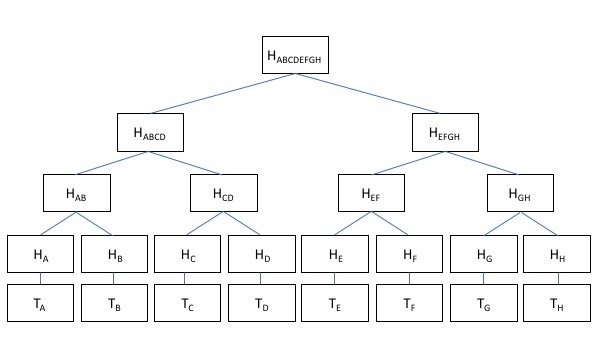
\includegraphics[scale=0.60]{MerkleTree.jpg}%
\caption{Abbildung zeigt einen Merkle Tree (Quelle https://www.investopedia.com/terms/m/merkle-tree.asp)}%
\label{fig:merkletree}%
\end{figure}

\section{Proof-of-Work (Hashcash)}\label{basic_HashCash}
Das Proof-of-Work Konzept wurde anf�nglich gegen denial-of-service Attacken oder f�r die Abwehr von Spam beim Email Verkehr entwickelt. Der Erfinder Adam Back nannte dieses System auch �Hashcash�.~\cite{je:hashcash} Damit eine Person, die dieses Konzept nutzt, beispielsweise eine Email versenden kann muss sie vorher einen kleinen Aufwand betreiben. Dies k�nnte eine einfache mathematische Formel sein. Bei erfolgreicher Berechnung ist die Email freigegeben. Da eine Vielzahl dieser kleinen Aufw�nde sich zu einem gro�em Rechenaufwand aufstaut und da die Komplexit�t der Aufw�nde mit jeder erfolgreichen Abarbeitung steigt, wird in der Schlussfolgerung das schnelle Versenden vieler aufeinander folgender Emails verhindert.

\section{Internet of Things (IoT)}
Das Internet of Things (deutsch: Internet der Dinge) beschreibt die Verkn�pfung von Ger�ten und Sensoren, die vorher eigenst�ndig und isoliert waren, mit dem Internet. Damit ist es ihnen m�glich Daten untereinander auszutauschen indem sie ihre eigenen Daten �bertragen und externe Daten anfordern. So lassen sich die Ger�te �ber das Internet gleichzeitig von Menschen oder anderen Maschinen fernsteuern. Mit diesem Begriff wird die Idee eingeleitet, dass die Nutzer des Internets nicht ausschlie�lich Menschen sind, sondern zunehmend auch �Dinge� (Things).

Im privaten Gebrauch werden als Beispiele allt�gliche Ger�te aufgef�hrt, die durch die Vernetzung im Internet mit anderen Ger�ten das Leben des Nutzers komfortabler machen oder auf sonstige Weise positiv beeinflussen. Ein Beispiel w�re die Hausautomation mit Sicherheitskameras, die, wenn etwas verd�chtiges ermittelt wird, sofort den Hauseigent�mer �ber das Internet warnen und das Videomaterial live auf dem Smartphone �bertragen.

Das Internet der Dinge l�sst sich auch im industriellen Bereich anwenden. So lassen sich Herstellungsprozesse durch die Vernetzung von Sensoren, Anlagen und Maschinen so automatisieren, dass der Prozess effizienter und menschliche Hilfe immer mehr obsolet wird. 

\section{Industrie 4.0}
In diesem Zusammenhang f�llt oft der Begriff Industrie 4.0. Damit ist eine vierte industrielle Revolution gemeint. Kurz beschrieben geht die erste industrielle Revolution mit der Mechanisierung einher, die zweite mit der Massenfertigung von Produkten mittels Flie�b�ndern und Fabriken, und die dritte mit der Automatisierung von Arbeitsschritten mittels Maschinen. Insofern handelt es sich bei Industrie 4.0 um die Vernetzung der automatisierten Arbeitsschritte, sodass sie autonom miteinander kommunizieren k�nnen und sich dem n�chsten Arbeitsschritt anpassen k�nnen.\footnote{Bezogen von https://www.yokogawa.com/de/loesungen/industrie-4-0.htm} 

\section{Trits, Trytes \& Tryte-Alphabet}\label{grundlagen:tritsundtrytes}
Das Tern�re System ist eine Alternative zu dem Bin�ren System, mit dem Unterschied dass das Tern�re System die Basis 3 hat. Ein Trit kann drei verschiedene Werte annehmen. Es ist die kleinste Einheit in dem Tern�ren System. Die Werte belaufen sich auf -1, 0 oder 1. Drei Trits ergeben ein Tryte. Ein Tryte kann $3^3 = 27$ Zust�nde annehmen. Um die Lesbarkeit einer l�ngeren tern�ren Zahl zu verbessern wurde von der IOTA-Foundation das sogenannte "`Tryte-Alphabet"' erstellt. Es besteht aus den 26 Zeichen des Alphabetes in Gro�buchstaben (A-Z) und der Zahl $9$. Jedes Zeichen repr�sentiert den Wert eines Tryte.

\begin{table}[H]
\centering
	\begin{tabular}{c|c}
		\begin{tabular}{P{1.8cm}|P{1.8cm}|P{1.8cm}}
			Tryte & Dezimal & Buchstabe \\
			\hline
			0, 0, 0 & 0 & 9 \\
			\hline
			1, 0, 0 & 1 & A \\
			\hline
			-1, 1, 0 & 2 & B \\
			\hline
			0, 1, 0 & 3 & C \\
			\hline
			1, 1, 0 & 4 & D \\
			\hline
			-1, -1, 1 & 5 & E \\
			\hline
			0, -1, 1 & 6 & F \\
			\hline
			1, -1, 1 & 7 & G \\
			\hline
			-1, 0, 1 & 8 & H \\
			\hline
			0, 0, 1 & 9 & I \\
			\hline
			1, 0, 1 & 10 & J \\
			\hline
			-1, 1, 1 & 11 & K \\
			\hline
			0, 1, 1 & 12 & L \\
			\hline
			1, 1, 1 & 13 & M \\
		\end{tabular}&
		\begin{tabular}{P{1.8cm}|P{1.8cm}|P{1.8cm}}
			Tryte & Dezimal & Buchstabe \\
			\hline
				&	&	\\
			\hline
			-1, -1, -1 & -13 & N \\
			\hline
			0, -1, -1 & -12 & O \\
			\hline
			1, -1, -1 & -11 & P \\
			\hline
			-1, 0, -1 & -10 & Q \\
			\hline
			0, 0, -1 & -9 & R \\
			\hline
			1, 0, -1 & -8 & S \\
			\hline
			-1, 1, -1 & -7 & T \\
			\hline
			0, 1, -1 & -6 & U \\
			\hline
			1, 1, -1 & -5 & V \\
			\hline
			-1, -1, 0 & -4 & W \\
			\hline
			0, -1, 0 & -3 & X \\
			\hline
			1, -1, 0 & -2 & Y \\
			\hline
			-1, 0, 0 & -1 & Z \\
		\end{tabular}
	\end{tabular}
\caption{Das Tryte Alphabet}
\label{tab:comparison}
\end{table}

\section{Distributed Ledger}
Eine Distributed Ledger (w�rtlich "`verteiltes Kontobuch"') Technologie (kurz DLT) kann sich wie ein �ffentlich einsehbares Kontobuch vorgestellt werden. Bei handels�blichen zentralen Transaktionen kann der Zahlende sich seines Handels zwar bewusst sein, jedoch nicht �ber den Status des Eingangs bei dem Zahlungsempf�ngers. Des weiteren hat der Zahlungsempf�nger keine Einsicht in die Verf�gbarkeit des Geldes oder des zu transferierenden Gegenstandes des Zahlenden. Der Handelsgegenstand kann in einer weiteren Transaktion bereits reserviert sein. Bei zentralisierten Handelsauftr�gen garantiert eine dritte Partei die Richtigkeit des Handels. Dabei wird das Vertrauen jedoch in diese vorausgesetzt. Eine DLT l�st dieses Problem, indem die Richtigkeit eines Handels nicht durch zentrale Parteien versichert wird, sondern durch systemimmanente Prozesse. Es besteht ein Konsens �ber die Richtigkeit der Daten, da sie dem System unabh�ngig und frei zur Verf�gung stehen. Dar�ber hinaus sind die get�tigten Handelsauftr�ge anonymisiert �ffentlich einsehbar und nicht auf die Handelsparteien zur�ckzuf�hren. Die Richtigkeit basiert nicht l�nger auf dem Vertrauen in eine Zentrale Partei, sondern wird durch den Konsens des Systems gew�hrleistet.

Eine DLT zeichnet den gesamten Handelsverlauf auf. Jeder Handel kann auf den Ursprung zur�ckverfolgt werden. Dem Handelspartner ist es ein Leichtes, den Verlauf eines Transaktionswertes nachzuweisen, indem er die Historie dessen zur�ckverfolgt.\footnote{Daten bezogen von: https://www.bafin.de/SharedDocs/Veroeffentlichungen/\\DE/Fachartikel/2016/fa\_bj\_1602\_blockchain.html}

\section{Hash}
Ein Hash stellt durch einen Wert einen anderen Wert dar. Er wird f�r verschiedene Zwecke genutzt. In der Computer Wissenschaft ist es ein Mittel um Beispielsweise Dateien zu komprimieren, Daten zu indizieren oder um eine Kryptographie zu realisieren. In der Kryptographie wird der Hash bevorzugt genutzt, da er Daten maskiert. Diese Eigenschaft resultiert aus der besonderen Beschaffenheit, dass der urspr�ngliche Wert eine Hashes in der Regel nicht wiederherstellbar ist, diesen jedoch repr�sentiert. \footnote{Daten bezogen von: https://techterms.com/definition/hash}

\section{Wallet}
Die Wallet ist der Verweis auf den eigenen Wertbestand und der Begriff wird oft in Zusammenhang mit Kryptow�hrungen genutzt. Technisch gesehen ist eine Wallet (Brieftasche) nicht der Ablageort der W�hrung wie es der Name f�lschlicherweise suggeriert. Bei der Kryptow�hrung Bitcoin verweist der private Schl�ssel auf die entsprechenden Geldeinheiten. Dieser ist nichts anderes als eine sehr gro�e Zahl und ohne den Zugang zu der Bitcoin-Blockchain ist es nicht m�glich den hinterlegten Wert zu erfahren. In diesem Zusammenhang wird der Begriff Wallet auch f�r die Software verwendet, die das Zusammenspiel des privaten Schl�ssels mit dem entsprechenden Distributed Ledger abwickelt. \footnote{Daten bezogen von: https://bitcoin.org/en/vocabulary\#wallet}

\section{Restful API}\label{RestfulAPI}
REST steht f�r Representational State Transfer Architektur und beschreibt ein Protokoll welches den Standart f�r heutige Web-Anwendungen setzt. Auf Anfrage eines Clients sendet der auf REST basierende Server eine Repr�sentation einer Ressource. Die Ressource selbst ist dabei nicht an einen Typ gebunden und kann jedes denkbares digitales Datum sein. Die Anfragen die dem Server gesendet werden k�nnen verschiedene Aufgaben erf�llen. So w�re im Beispiel eines Online-Shops das Speichern von Kundendaten auf dem Server realisierbar. Eine wichtige Eigenschaft der auf REST basierenden Server ist, dass sie den Status des anfragenden Clients nicht speichern oder dieser von Belangen sei. Alle gesendeten Anfragen m�ssen die notwendigen Daten enthalten um von dem Server entsprechend verarbeitet zu werden.~\cite{je:rest}

\section{Zusammenfassung}
Die benannten Grundlagen vermitteln ein Verst�ndnis f�r die kommende Ausarbeitung. Die allgemeine Funktionsweise eines Respberry Pis umfasst sowohl die physischen Komponenten, wie beispielsweise die korrekte Einrichtung des Steckbrettes, als auch die technische Programmierung der einzelnen GPIO - Pins. Um eine Grundlage in der Kryptographie zu vermitteln, ist die Funktion eines Merkle - Trees, der Aufbau eines Hashes sowie das Proof-of-Work - Konzept von essentiellem Belangen. Das Kapitel Grundlagen umfasst neben diesen Informationen weiteres Basiswissen �ber die allgemeine Definition von Distributed Ledger Architekturen und des Internet of Things (IoT).
\part{Theoretischer Teil}
\chapter{Einf�hrung}
- welche Distributed Ledger Technologien werden verwendet\\
- warum werden sie verwendet\\
- welche Kryptow�hrungen werden als beispiel f�r die ausgew�hlten Distributed Ledger technologien genommen\\
  - Bitcoin f�r blockchain und IOTA f�r tangle\\

\chapter{Funktion}
Die Funktion von Distributed Ledger Architekturen wird �ber verschiedene Kryptographien und Techniken erm�glicht. Das kommende Kapitel stellt die Funktion dieser Konzepte anhand der jeweiligen Umsetzung in Bitcoin und IOTA detailliert dar.

\section{Bitcoin}
Bitcoin ist ein Distributed Ledger Protokoll das erstmalig Geldtransfer �ber eine dezentrale, anonyme �bereinstimmung der Richtigkeit verf�gt. Diesen Konsens erreicht es �ber die implementierte Blockchain, die wie ein global einsichtiges Kassenbuch funktioniert. Die Blockchain kann auf verschiedene Art und Weise genutzt und entwickelt werden. Sie erm�glicht es �ber das Internet Werte auszutauschen ohne von einem Mittelsmann abh�ngig zu sein~\cite{je:whatIsBitcoin}. Durch kryptographische Techniken sind Daten die in die Blockchain gelangen nur durch sehr gro�en Aufwand manipulierbar, was sie f�r das Speichern von sensiblen Daten attraktiv macht. Im Folgenden wird die grundlegende Funktion der Blockchain sowie dessen Einsatz bei Bitcoin sachlich untersucht.

\subsection{Allgemeine Funktion}
F�r die gegenw�rtige Funktion von Bitcoin und dessen Blockchain sind zwei elementare Techniken notwendig. Zum einen ist das die Public-Key-Kryptographie zum anderen die kryptographischen Hashfunktionen.

Bei der Public-Key-Kryptographie resp. digitalen Signatur erstellt der Sender einer Nachricht ein Schl�sselpaar bestehend aus einem privaten sowie einem �ffentlichen Schl�ssel. Die beiden Schl�ssel haben zwei erg�nzende Funktionen. Der Autor der Nachricht verwendet den privaten Schl�ssel um diesen mit seinen Informationen zu verbinden und dadurch zu signieren. Die signierten Daten werden gemeinsam mit dem �ffentlichen Schl�ssel an den Empf�nger weitergegeben. Dank des �ffentlichen Schl�ssel ist es dem Empf�nger m�glich die Daten zu authentifizieren. Des Weiteren ist durch die Verkn�pfung der Daten mit dem privaten Schl�ssel die inhaltliche Integrit�t vor Manipulation gesch�tzt.

Durch kryptographische Hashfunktionen entstehen aus Zeichenketten mit variabler L�nge Zeichenketten fester L�nge. Diese Zeichenketten sind �deterministisch�. Die gleichen Eingangsdaten werden nach der Hash-Berechnung immer den gleichen Hash verursachen. Ver�nderte Eingangsdaten f�hren zu einem stark abweichenden Hash.

Au�erdem gibt es drei weitere nennenswerte Eigenschaften von Hashfunktionen. Zum Einen ist es nahezu unm�glich durch den Hash die anf�nglichen Daten wiederherzustellen. Des Weiteren ist es nahezu unm�glich mit abweichenden Eingangsdaten denselben Hash zu generieren. Zuletzt ist es nahezu unm�glich zwei verschiedene Eingangsdaten zu finden aus denen sich derselbe Hashwert ergibt.~\cite{je:whatIsHash}

\subsection{Privater \& �ffentlicher Schl�ssel}\label{ECC}
Der private Schl�ssel in Bitcoin kennzeichnet den Besitz der �bertragenden BTCs (Geldeinheit). Sollte der Schl�ssel verloren gehen, ist es nicht m�glich die BTCs, die dem privaten Schl�ssel zugeordnet sind, wiederherzustellen. Der �ffentliche Schl�ssel wird f�r die Verifikation einer Transaktion ben�tigt, da er durch den privaten Schl�ssel generiert wurde. Man kann durch den �ffentlichen Schl�ssel, nach heutigem Stand, nicht den privaten Schl�ssel erraten. Dieses Ziel wird durch die folgende Kryptographie erreicht:

\paragraph{Endliche Felder}
Ein endliches Feld ist eine Gruppe aus Zahlen, das, wie der Name suggeriert, endlich ist. Ein endliches Feld, das mit Zahlen des Modulo P gebildet wird, bei dem P eine Primzahl ist, f�hrt zu n�tzlichen Funktionen in der Kryptographie.

\paragraph{Elliptische Kurven}
In der Mathematik sind elliptische Kurven aufgrund ihrer Eigenschaft, mathematische Gruppen zu sein, interessant. Eine elliptische Kurve wird nach der folgenden Formel gebildet:

\begin{equation*}
	\{(x,y) \in \mathbb{R}^2 \mid y^2 = x^3 + ax + b,\, 4a^3 + 27b^2 \neq 0 \} \cup \{ 0 \}
\end{equation*}

F�r jeden Punkt der elliptischen Kurve gelten die Gesetze der Kommutativit�t, Assoziativit�t und Distributivit�t. Dar�ber hinaus gelten weitere, f�r elliptische Kurven spezifische, Regeln:

\begin{description}
	\item[-] Die Inverse -P eines Punktes P kann durch das Spiegeln des Punktes P an der x-Achse bestimmt werden.
	\item[-] Wenn zwei Punkte (P, Q) einer elliptischen Kurve bekannt sind, kann immer auch ein dritter Punkt (R) bestimmt werden. Die Addition der drei Punkte ergibt in jedem Fall $ P + Q + R = 0 $. Insofern w�re die Rechnung der Punkte zur Bestimmung von Punkt R: $ P + Q = -R $. Punkt -R ist die Inverse von Punk R gespiegelt an der x-Achse.
\end{description}

Eine Formel die diese beiden Konzepte, der elliptischen Kurven und der endlichen Felder, vereint sieht wie folgt aus:

\begin{equation*}
	\{(x,y) \in \mathbb{R}^2 \mid y^2 \equiv x^3 + ax + b\, (mod\, p),\, 4a^3 + 27b^2 \not\equiv 0\, (mod\, p)\} \cup \{ 0 \}
\end{equation*}
Gruppe aus den Reellen Zahlen der elliptischen Kurven des modulo P \cite{je:ellipticCurve}

Dank des Moduls p befindet sich die Gleichung in einem endlichen Feld. Eine elliptische Kurve die sich in einem endlichen Feld befindet ist weiterhin in eine mathematische Gruppe. Alle Formeln k�nnen wie zuvor beschrieben angewandt werden.

Tritt der Fall ein, dass Punkt P sich wie eine Tangente zu der elliptischen Kurve verh�lt, wird das sogenannte Prinzip der Punktdopplung genutzt: 
\begin{equation*}
	P + Q = -R;\: Q = P \rightarrow 2P = -R
\end{equation*}

Es ist m�glich den Punkt P um eine beliebige Anzahl x zu skalieren um einen Punkt R zu erreichen.

\begin{equation*}
	xP = R
\end{equation*}

Da sich Punkt P in einem endlichen Feld befindet, wird durch ein, abh�ngig des Punktes P, gew�hlter bestimmter Skalar x daf�r Sorgen, dass das Produkt auf die Ausgangsposition P verweist. Dieses Prinzip l�sst sich gut durch den Zeiger einer Uhr verdeutlichen. Die Ausgangsuhrzeit ist 3 Uhr. Der Zeiger wandert in drei Stunden Schritten voran. Nach vier Schritten zeigt der Stunden Zeiger erneut auf die Ausgangsuhrzeit 3 Uhr.

Es entsteht eine Untergruppe die durch den Punkt P definiert ist. Die Ordnung n dieser Gruppe P wird so gew�hlt dass nP = 0 ist. In dem Beispiel der Uhrzeit entspricht die Ordnung n = 4 denn $4(3)\: mod(12) = 0$.

Bitcoin nutzt folgende Werte f�r die elliptische Kurven Kryptographie:

\begin{description}
	\item[1.] Der prim�re Wert des Moduls zum Bestimmen des endlichen Raumes entspricht: $2^{256} - 2^{32} - 2^9 - 2^8 - 2^7 - 2^6 - 2^4 - 1 \rightarrow$ FFFFFFFF FFFFFFFF FFFFFFFF FFFFFFFF FFFFFFFF FFFFFFFF FFFFFFFE FFFFFC2F (hex).
	\item[2.] Die elliptische Kurve wird mit den Parametern $a=0$ und $b=7$ gebildet.
	\item[3.] Die Basis der Untergruppe P betr�gt in hexadezimal: 04 79BE667E F9DCBBAC 55A06295 CE870B07 029BFCDB 2DCE28D9 59F2815B 16F81798 483ADA77 26A3C465 5DA4FBFC 0E1108A8 FD17B448 A6855419 9C47D08F FB10D4B8 (hex).
	\item[4.] Die Ordnung n der Untergruppe P betr�gt in hexadezimal: FFFFFFFF FFFFFFFF FFFFFFFF FFFFFFFE BAAEDCE6 AF48A03B BFD25E8C D0364141 (hex).
\end{description}

Der private Schl�ssel ist eine Zahl zwischen 1 und der angegebenen Ordnung. Um den �ffentlichen Schl�ssel zu errechnen, wird der private Schl�ssel mit dem Basispunkt der Untergruppe P multipliziert. Das Ergebnis $mod$ des prim�ren Wertes des Moduls ergibt den �ffentlichen Schl�ssel. Dieser entspricht einem Wert der durch nahezu unendlich M�glichkeiten erreicht werden kann. Nur der Besitzer des privaten Schl�ssels kann diesen Wert gezielt reproduzieren.~\cite{je:ellipticCurve}

\subsection{Transaktionen}
Um eine Transaktion im Bitcoin Netzwerk zu veranschaulichen wird ein fiktives Beispiel herangezogen. Alice m�chte an Bob zwei Bitcoins (BTC) versenden. Es existieren jedoch keine Konten oder Kontost�nde, sondern ausschlie�lich die �ffentliche Liste aller jemals get�tigten Transaktionen, also die Bitcoin - Blockchain selbst, sowie die Hashwerte der einzelnen �ffentlichen Schl�ssel denen die existierenden Transaktionen zugeordnet werden. Aufgrund der vergangenen Transaktionen kann der Wertbestand an BTCs des zugeh�rigen privaten Schl�ssels ermittelt werden. Mithilfe einer digitalen Software (Wallet) kann dieser Wertbestand des privaten Schl�ssels eingesehen und neue Transaktionen eingereicht werden. Um eine Transaktion zu veranlassen werden mithilfe des privaten Schl�ssels die zur�ckliegenden eingegangenen Transaktionen signiert und zusammen mit der ausgehenden Transaktion an das Bitcoin Netzwerk versandt. Dies entspricht in dem anf�nglichen Beispiel einer Auflistung aller Transaktionen in denen Alice involviert war, sowie Alice� Intention zwei BTCs an den �ffentlichen Schl�ssel von Bob zu senden. 

Diese Nachricht gelangt an einen Netzknoten der �ber verschiedene Ressourcen verf�gt. Neben einer aktuellen und vollst�ndigen Kopie der Blockchain, einen Cachespeicher ("`Unspent Transaction Output"' UTXO), der Transaktionswerte der Blockchain enth�lt die noch nicht f�r neue Transaktionen verwendet wurden, existiert noch eine Datenbank mit unbest�tigten Transaktionen. In diesem Netzknoten wird die Legitimit�t von Alice� Transaktion �berpr�ft, indem zum einen ihre Liquidit�t aufgrund ihrer bisherigen Transaktionen, sowie gleichzeitig ihre Signatur anhand des �ffentlichen Schl�ssels, best�tigt wird. Mithilfe der UTXO wird au�erdem gepr�ft, ob die genutzten BTCs nicht bereits anderweitig reserviert wurden. Wenn dies fehlerfrei geschieht, wird die unbest�tigte Transaktion in die daf�r eingerichtete Datenbank aufgenommen. Der Netzknoten meldet diese eingereichte Transaktion an m�glichst viele weitere Netzknoten weiter, die wiederum die Daten nach dem erkl�rten Schema �berpr�fen und anschlie�end in die Datenbank der unbest�tigten Transaktionen aufnehmen.~\cite{je:blockchainBasics}

\subsection{Mining}
Das Bitcoin-Netzwerk verf�gt �ber zwei Arten von Netzwerkknoten. Einer ist ausschlie�lich f�r das zuvor genannte Verifizieren und Speichern der eingehenden Transaktionen sowie dessen Weiterleitung an weitere Netzknoten zust�ndig. Der zweite ist dar�ber hinaus bef�higt neue Bl�cke in der Blockchain zu speichern. Dieser sogenannte �Mining-Netzknoten� speichert zun�chst unbest�tigte Transaktionen in einem Block zusammen. Dieser Block besitzt zus�tzlich einen Blockheader, der f�r die kommende Abspeicherung in der Blockchain essentiell ist.

Es ergeben sich ab diesem Zeitpunkt einige Problematiken. Aufgrund von Verz�gerungen im Netzwerk oder m�glichen Ausf�llen sind einige Netzknoten aktueller. Dies f�hrt dazu, dass verschiedene Transaktionen, welche sich voneinander unterscheiden, in den einzelnen Netzknoten existieren. Au�erdem k�nnen b�sartige Absender gef�lschte Transaktionen weiterleiten, welche dieselben Wert-Ressourcen aufweisen. Bitcoin verwendet f�r diese Problematiken die Proof-Of-Work (PoW) Technologie. In der Regel wird diese Technik f�r das Verhindern von missbr�uchlicher Benutzung von Diensten eingesetzt. Damit ein Dienst genutzt werden kann muss bei dieser Technik ein gewisser Aufwand erbracht werden. Im Falle der Bitcoin-Blockchain muss gem�� dieses Schemas eine rechenintensive Aufgabe gel�st werden. Der Block-Header ergibt einen gewissen Hashwert. Dieser muss solange manipuliert werden bis das Ergebnis unterhalb eines gewissen Zielwertes liegt. Diese partielle Hashinversion beruht auf dem Hashcash-Prinzip von Adam Back (siehe Grundlagen Kapitel \ref{basic_HashCash} auf Seite \pageref{basic_HashCash} ). Der Hash entspringt dem Block-Header und wird aus einer Referenz zum vorherigen Block, einem Zeitstempel, dem Zielwert des Hash-R�tsels, dem Top Hash eines Merkle-Trees, welcher alle Transaktionen durch aufeinander aufbauende Hashes zusammenfasst, sowie einer variablen Zeichenfolge (Nonce) errechnet. Die Nonce wird so oft ge�ndert bis der Hashwert unterhalb des Zielwertes liegt. In anderen Worten muss dieser mit einer gewissen Anzahl von Nullen beginnen. Der erste Mining-Netzknoten der dieses R�tsel l�st versendet seinen Block an das Netzwerk. Dort wird der Block ebenfalls auf Validit�t gepr�ft und bei Erfolg in die eigene Blockchain integriert.

In 1,69\% der F�lle, finden zwei Netzknoten zu nahezu der gleichen Zeit eine L�sung des Hash-R�tsels und versenden ihre jeweiligen Bl�cke. In diesem Fall erhalten unabh�ngige Netzknoten verschieden Versionen der Blockchain. Infolgedessen teilen sich die Netzknoten auf. Dieses Ph�nomen ist als Gabelung bekannt. Die jeweiligen Netzknoten arbeiten weiter auf Grundlage ihrer bekannten Blockchain bis zu dem Moment bei dem sie �ber eine l�ngere Blockchain Version informiert werden. Tritt dieser Fall ein, wird die bekannte Blockchain durch die l�ngere ausgetauscht. Sollte die l�ngere Version einige Transaktionen der zuvor bekannten Blockchain nicht enthalten, werden diese wieder in die Datenbank der nicht best�tigten Transaktionen aufgenommen. Momentan wird ca. alle zehn Minuten ein neuer Block in die Blockchain aufgenommen. Damit sich diese Zeitspanne weiter in einem angemessenen Rahmen befindet, wird stetig die Komplexit�t des Hash-R�tsels angepasst. F�r das Finden der L�sung eines Hash-R�tsels und das erfolgreiche Integrieren eines neuen Blockes in der Blockchain, erh�lt der Mining-Netzknoten eine gewisse Menge an BTCs, wodurch neue BTCs erzeugt werden.~\cite{je:blockchainBasics}

\section{IOTA}
IOTA ist ein Distributed Ledger Protokoll, welches eine grenzenlose Skalierbarkeit des eigenen Netzwerkes zul�sst. Dies wird durch die Eigenschaft erm�glicht, das der Benutzer und der Miner nicht l�nger voneinander getrennt sind. In IOTA wird das Prinzip der durch Bitcoin bekannten Blockchain umgedacht. Transaktionen werden nicht l�nger in einem Block gespeichert, sondern �ber ein Netz aus Transaktionen verteilt. In diesem Netz best�tigen sich die jeweiligen Transaktionen gegenseitig ihre Richtigkeit. Dieses Netz wird Tangle genannt und kann sich wie ein "`Directed Acyclic Graph"' vorgestellt werden. Die folgende Untersuchung liefert einen sachlichen Einblick in die Funktion IOTAs und der implementierten Tangle.

\subsection{IOTA Seed}
Der IOTA Seed ist essentiell wichtig f�r die Funktion von IOTA. Er fungiert als "`Kontonummer"' und verweist auf die Menge an IOTAs die dem Konto zugeordnet werden (das IOTA-Wallet). Wenn der Besitzer des Seeds eine Transaktion durch die IOTA-Tangle veranlassen m�chte, wird mit Hilfe von kryptographischen Hashfunktionen eine Adresse aus dem Seed erstellt. Diese Adresse kann nun genutzt werden um IOTAs zu empfangen oder, sollte sie bereits einen Wert besitzen, zu versenden. Adressen k�nnen nur durch den Seed generiert werden und es ist (technisch) unm�glich von der Adresse den Seed wiederherzustellen. Ein Seed besteht aus 81 Trytes die dank des von der IOTA-Foundation zur Verf�gung gestellten "`Tryte-Alphabet"' durch die 26 Gro�buchstaben A-Z des Alphabets und der Zahl 9 dargestellt werden. \footnote{Diese Vorgaben sind von der IOTA Foundation ver�ffentlicht: https://iota.readme.io/docs/seeds-private-keys-and-accounts}

\subsection{Tangle}\label{grundlagen:tangle}
Bei Tangle handelt es sich um ein Distributed Ledger Software Protokoll, welches sich grundlegend von Blockchain unterscheidet. Die Tangle-Technologie wird von den Entwicklern als n�chste evolution�re Weiterentwicklung der Blockchain beschrieben ~\cite{je:theTangle}. Die Technologie nimmt sich den Schw�chen der Blockchain an und integriert L�sungen f�r diese. Konzeptionell bedeutet dies, dass die heterogene Unterscheidung von Minern und Usern in Blockchains homogenisiert werden soll, indem Transaktionen von Nutzern verifiziert werden sollen, die selber eine Transaktion veranlassen m�chten. So l�st sich das Problem der Skalierung und zugleich fallen die Transaktionsgeb�hren weg. Letzteres ist m�glich, da es zwingend notwendig ist, andere Transaktionen zu verifizieren, falls eine eigene Transaktion aufgegeben werden soll. So "`zahlt"' der Nutzer die Geb�hren mit Rechenleistung.

Tangle wurde von der IOTA-Foundation entwickelt und kommt in der gleichnamigen Kryptow�hrung IOTA zum Einsatz.

Anders als bei Blockchain ist es nicht m�glich, neue Tokens zu "`minen"' (bedeutet: herzustellen). Es besteht seit der Entwicklung ein fester Betrag an verf�gbaren Tokens von genau 2.779.530.283 MIOTA (1 MIOTA = 1.000.000 IOTA) \footnote{Daten bezogen von: https://coinmarketcap.com/currencies/iota/}. Die Tangle richtet sich nach einem Mathematischen Konzept, dem Directed Acyclic Graph. Mit diesem Konzept speichert IOTA die Transaktionen.
Eine Transaktion muss von einem Node aufgegeben werden. Sobald eine Transaktion nicht verifiziert werden kann, kann die urspr�ngliche Transaktion nicht ausgehen.~\cite{je:theTangle}

\subsection{Directed Acyclic Graph}
Die IOTA-Tangle ist aufgebaut in Form eines "`Directed Acyclic Graph"' (DAG) was in diesem Kontext bedeutet, dass sie sich in eine Richtung bewegt und niemals kreisf�rmig ist. Damit eine neue nicht verifizierte Transaktion in die Tangle aufgenommen werden kann, ist neben dem Proof-of-Work eine Verifikation von zwei ebenfalls nicht verifizierten Transaktionen notwendig. Diese beiden Transaktionen werden in dem Transaktions-Bundle abgespeichert und sind dementsprechend referenziert. Da nur nicht verifizierte Transaktionen in diesem Prinzip verwendet werden, entspricht der entstehende Graph eines DAG. \footnote{Daten bezogen von: https://www.forbes.com/sites/shermanlee/2018/01/22/explaining-directed-acylic-graph-dag-the-real-blockchain-3-0}

\subsection{Transaktion}
Eine Transaktion in IOTA besteht aus mehreren Hashes und Werten, die jeweils untereinander eine verschiedene Aufgabe erf�llen. In den folgenden Abschnitten werden diese detailliert aufgef�hrt.

\paragraph{signatureMessageFragment}
Sollte die Transaktion eine ausgehende Zahlung sein, wird dieses Feld ben�tigt um die Signatur des privaten Schl�ssels zu enthalten. Die L�nge der Signatur ist davon abh�ngig, mit welcher Sicherheitsstufe diese Transaktion gehasht wird. Sollte die Sicherheitsstufe 2 oder 3 sein, wird eine weitere wertlose Transaktion ben�tigt. Diese speichert in dem noch freien Signature Message Fragment den Rest der Signatur der vorangehenden ausgehenden Zahlung.

Sollte jedoch die Signatur des privaten Schl�ssels nicht erforderlich sein, verbleibt dieses Feld leer und kann f�r das �bertragen einer Nachricht genutzt werden.
Diesem Feld werden 2187 Trytes reserviert.

\paragraph{hash}
In diesem Feld wird der "`transaction Hash"' nach dem Finden der "`nonce"' und dem Proof-of-Work abgespeichert. Die L�nge betr�gt 81 Trytes.

\paragraph{address}
Die Adresse der Transaktion wird erneut f�r verschiedene Aufgaben verwendet, die sich aus der Art der Transaktionen definieren. Sollte eine Zahlung durchgef�hrt werden, wird in diesem Feld die Adresse des Empf�ngers angegeben. Handelt es sich jedoch um eine urspr�ngliche Geldeingangs-Adresse so ist hier eine Adresse aufgef�hrt die aus einem private Key des Besitzer's Seed erstellt wurde.
F�r dieses Feld sind 81 Trytes reserviert.

\paragraph{value}
Der Wert einer Transaktion definiert dessen Art. Sollte dieser Wert positiv sein, handelt es sich um eine zahlende Transaktion (Output). In dem Feld "`Address"' wird sich in diesem Fall die Adresse des Empf�ngers befinden und das Feld "`Signature Message Fragment"' ist entweder leer oder beinhaltet eine benutzerspezifische Nachricht.

Sollte der Wert negativ sein handelt es sich bei der Transaktion um eine empfangene Transaktion (Input). Das Feld "`Address"' enth�lt entsprechend eine Adresse die dank des Seeds und einem daraus entstandenen private Key generiert wurde. Eine eingehende Transaktion enth�lt einen negativen Wert, um den positiven Wert einer ausgehende Zahlung im Bundle zu rechtfertigen. Zwangsl�ufig wurde diese Adresse zuvor von einer fremden IOTA-Transaktion als Empf�nger Adresse genutzt.

Um den Besitz des entsprechenden privaten Schl�ssels zu beweisen, wird in dem "`Signature Message Fragment"' die Signatur durch den privaten Schl�ssel abgespeichert. Sollte die Sicherheitsstufe gr��er als 1 sein, werden weitere Transaktionen ben�tigt, um die gesamte Signatur zu speichern.

Tr�gt dieses Feld keinen Wert und entspricht 0, handelt es sich bei der Transaktion entweder um das Versenden einer einfachen Nachricht an eine Empf�ngeradresse oder wird genutzt um die Signatur einer vorangehenden Transaktion zu speichern.

F�r dieses Feld wurden 27 Trytes reserviert.

\paragraph{obsoleteTag}
Der obsolete Tag enth�lt einen vom Benutzer definierten Tag. Dieser k�nnte in zuk�nftigen IOTA - Iterationen entfernt werden.
Die reservierte L�nge dieses Feldes betr�gt 27 Trytes.

\paragraph{timestamp}
Der Zeitpunkt ist nicht verpflichtend und kann ausgelassen werden.
Ihm werden 9 Trytes reserviert.

\paragraph{currentIndex}
Dieses Feld zeigt die momentane Position im Bundle.
Ihm werden ebenfalls 9 Trytes reserviert.

\paragraph{lastIndex}
Dieses Feld f�hrt den Index der letzten Transaktion des umfassenden Bundles auf und liefert dementsprechend die L�nge dessen.
Reserviert werden erneut 9 Trytes.

\paragraph{bundle}
Dieses Feld enth�lt den Hash des umfassenden Bundles. Er wird genutzt um alle Transaktionen dieses Bundles zu gruppieren. Jede Transaktion in einem Bundle enth�lt in diesem Feld denselben entsprechenden Bundle Hash. Das Feld umfasst 81 Trytes L�nge.

\paragraph{branch- \& trunkTransaction}
Diese beiden Felder sind jeweils 81 Trytes lang und enthalten zwei zuf�llig gew�hlte, nicht verifizierte Transaktionen aus der Tangle. Nicht verifizierte Transaktionen im Tangle werden "'Tips"' genannt. Jede Transaktion ist verpflichtet, zwei zuf�llig gew�hlte Tips in der Tangle zu verifizieren, um selbst als Tip aufgenommen zu werden.

\paragraph{tag}
Dieser Tag wird vom Benutzer gew�hlt und kann frei vergeben werden. Er kann die Suche einer Transaktion im Tangle unterst�tzen. Seine L�nge in der Transaktion betr�gt 27 Trytes.

\paragraph{attachmentTimestamp}
Dieses neun Trytes gro�e Feld beinhaltet den Zeitpunkt direkt nachdem der Proof-of-Work durchgef�hrt wurde. 

\paragraph{attachmentTimestampLowerBound \& attachmentTimestampUpperBound}
Diese beiden Felder zeigen ein Intervall auf in der die Aufnahme in die Tangle geschah. Sie sind jeweils 9 Trytes gro�.

\paragraph{nonce}
Die nonce ist ein besonders wichtiger Teil einer Transaktion, denn sie wird ben�tigt um den Proof-of-Work durchzuf�hren. Die L�nge dieses Feldes betr�gt 27 Trytes.

Rechnet man die L�ngen aller Felder zusammen, so erh�lt man die gesamte L�nge von 2673 Trytes. Dies ist die von der IOTA-Foundation vorgegebene L�nge die eine Transaktion haben soll. Die Art einer Transaktion bestimmt sich durch den Wert. Sollte eine Transaktion einen negativen Wert haben, so handelt es sich dabei um eine "`Input"' Transaktion. Bei einem positiven Wert, wird Balance an eine "`Output"' Adresse geschickt. Viele Felder tragen eine wichtige Aufgabe f�r die Aufnahme in der Tangle. So wird das Feld "`signatureMessageFragment"` entweder f�r benutzerspezifische Nachrichten genutzt oder, falls ben�tigt, f�r die Signatur.\footnote{Diese Vorgaben sind von der IOTA Foundation ver�ffentlicht: https://iota.readme.io/docs/the-anatomy-of-a-transaction}

\subsection{Proof-of-Work}
Um Transaktionen in die Tangle zu platzieren, sind keine Geb�hren notwendig. Das ist aufgrund zwei essentieller Eigenschaften m�glich. Zum Einen muss jede Transaktion zwei weitere nicht verifizierte Transaktionen best�tigen, des Weiteren wird mit Rechenleistung in Form eines Proof-of-Work die Transaktion beglaubigt. Im Detail l�uft dieses Verfahren wie folgt ab:
Nachdem alle Felder der Transaktion, bis auf die "`nonce"' und den Hash f�r  "`bundle"', einen Wert erhalten haben, wird mit Hilfe eines Algorithmus die nonce gesucht. Diese ist 27 Trytes lang. Sobald die nonce gefunden wurde, wird sie f�r die letzten 27 Trytes der insgesamt 2673 Trytes der Transaktion verwendet. Diese Trytes werden durch den Curl Hash Algorithmus zu einem 81 Trytes langen Hash umgewandelt. Der Hash wird im Anschluss in Trits umgerechnet. Am Ende der resultierenden 243 Trits soll eine Folge aus Nullen stehen. Die l�nge der Folge wird von der IOTA-Foundation vorgegeben. So m�ssen die letzten Trits der Trytes, eines Transaktions Hashes, momentan mindestens 14 mal Null in Folge f�r die Aufnahme in der Tangle und Neun mal Null in Folge f�r die Aufnahme in dem Testnetzwerk betragen. Diese Vorgabe wird "`Minimum Weight Magnitude (MWM)"' genannt. Der Vorgang wird sooft wiederholt bis das vorgegebene MWM erreicht ist. Grunds�tzlich kann die Aussage getroffen werden, dass mit einer steigenden MWM auch die Zeit, die f�r das Finden der passenden nonce ben�tigt wird, exponentiell ansteigt.

\subsection{Bundle}
IOTA ist nach einem Account - Schema aufgebaut, was genauer bedeutet, dass Adressen ben�tigt werden auf die Balance (der Fachausdruck des Geldwertes) eingegangen ist, um Balance weiter zu senden. Ein Bundle in IOTA umfasst in der Regel vier Transaktionen. Die erste Transaktion enth�lt die Adresse des Empf�ngers. Diese Transaktion wird mit einer positiven Balance versehen. In dem Bundle ist dies eine sogenannte "`Output"' - Transaktion. Daraufhin folgen in der Regel, abh�ngig von der gew�hlten Sicherheitsstufe, zwei Transaktionen. Jede dieser Transaktionen basiert auf der gleichen Adresse, auf der zuvor Balance eingegangen ist. In anderen Worten muss diese Adresse zuvor Teil einer "`Output"' - Transaktion gewesen sein. Es werden mehrere Transaktionen ben�tigt, da die Signatur des privaten Schl�ssels mit versandt wird. Diese Signatur vergr��ert sich, abh�ngig von der gew�hlten Sicherheitsstufe. Eine Transaktion, die sich einer Adresse bedient, die zuvor Balance empfing, nennt sich "`Input"' - Transaktion. Sollte die Balance der Input Transaktion nicht ausreichen um den Betrag der Output Transaktion zu decken, m�ssen weitere "`Input"' - Transaktionen angef�gt werden, die jeweils durch ihren privaten Schl�ssel signiert werden. Sollte die Balance der "`Input"' - Adressen den Wert der "`Output"' - Transaktion �berschreiten, wird der Restwert an eine "`Output"' - Adresse des Besitzers �bertragen. Solange der summierte Wert der "`Input"'-Adressen nicht �berschritten wird, k�nnen beliebig viele "`Output"'-Adressen einem Bundle angehangen werden.

Da Bundles atomar sind, werden entweder alle oder keine Transaktion verifiziert.

\subsection{Signatur}\label{OneTimeSignature}
Bei IOTA werden ausgehende Zahlungen (Output) mit zuvor eingegangenen Zahlungen (Input) durchgef�hrt. Um den Besitz des notwendigen Inputs nachzuweisen, verwendet IOTA die "`Winternitz One Time Signature"'. Diese Art der Signatur ver�ffentlicht einen Teil des privaten Schl�ssels und wird aus diesem Grund f�r den einmaligen Gebrauch von Signaturen verwendet. Um die Funktionsweise einer "`One Time Signature"' (kurz OTS) zu verdeutlichen, wird die �hnliche Lamport OTS in einem fiktiven Beispiel herangezogen.

Ein privater Schl�ssel besteht aus zwei gleichlangen Zahlenfolgen "`k1"' \& "`k2"'. Die L�nge des jeweiligen Schl�ssel Teils stimmt mit der L�nge der zu signierenden Nachricht �berein. In diesem Beispiel betr�gt die Schl�ssell�nge 512 (2x 256). Die Nachricht kann eine beliebige Zeichenkette sein, die bspw. durch den SHA-256 Hash Algorithmus zu einem Hash "`H"' mit der L�nge von insgesamt 256 Bits umgewandelt wurde. Der Wert eines Bits kann ausschlie�lich Null oder Eins betragen. In einer Schleife wird jeder Wert des Hashes durchlaufen. Betr�gt der Wert H(n) des Hashes an der Stelle n => H(n) = 0, so wird der Wert des ersten Schl�ssel Teils an selbiger Stelle f�r die Signatur Sig(n) = k1(n)  verwendet. Sollte jedoch der Wert H(n) des Hashes an der Stelle n => H(n) = 1 betragen, wird der Wert des zweiten Schl�ssel Teils in der Signatur Sig(n) = k2(n) verwendet. Nach dem erfolgreichen Durchlaufen des Hashes "`H"' wurde eine Signatur "`Sig"' mit einer L�nge von 256 angefertigt. Die Signatur enth�lt 50\% der Werte des privaten Schl�ssels.

Damit der Empf�nger die Signatur �berpr�fen kann, ben�tigt er den �ffentlichen Schl�ssel. Dieser ist bspw. ein, durch den SHA-256 Hash Algorithmus angefertigter, Hash "`pub"' des privaten Schl�ssels.
Der Empf�nger erh�lt die Nachricht, die Signatur �Sig� und den �ffentlichen Schl�ssel "`pub"'. Er wiederholt den Vorgang, den der Versender der Nachricht f�r die Signatur angewandt hat, mit dem �ffentlichen, mitgelieferten Schl�sselpaar "`pub1"' \& "`pub2"' anstatt des privaten Schl�sselpaars "`k1"' \& "`k2"'. Als Resultat erh�lt er eine gehashte Variante "`HSig"'. Sollte jeder Wert der "`HSig(n)"' identisch mit jedem Hash-Wert der Signatur "`SHA-256( Sig(n) )"' sein, ist die Integrit�t der Nachricht gew�hrleistet.~\cite{je:lamportSignature}

Sollte bei den kommenden Transaktionen erneut der gleiche private Schl�ssel zum Signieren herangezogen werden, wird bei jeder Signatur ein weiterer Teil des privaten Schl�ssels aufgedeckt. Ein b�swilliger Beobachter der Tangle k�nnte die Transaktionen abfangen und mittels Bruteforce-Attacken den gesamten privaten Schl�ssel aufdecken. Der Seed w�re weiterhin unbekannt, sollte der Adresse jedoch ein Wert hinterlegt sein, w�re der Angreifer in der Lage dar�ber zu verf�gen.

\section{Zusammenfassung}
Das Kapitel Funktion umfasst die detaillierte Funktionalit�t von den Kryptow�hrungen Bitcoin und IOTA. Die Kryptographie der privaten und �ffentlichen Schl�ssel der jeweiligen Technologien unterscheidet sich insofern, dass Bitcoin ausschlie�lich einen privaten Schl�ssel und den entsprechenden �ffentlichen Schl�ssel f�r das Erstellen und Bearbeiten einer Transaktion nutzt. IOTA hingegen generiert aus dem Seed mehrere private Schl�ssel dessen �ffentliche Schl�ssel als Adressen gelten. Bitcoin speichert Transaktionen in Bl�cken in der Blockchain, die durch "`minen"' circa alle 10 Minuten um einen weiteren Block verl�ngert wird und �ffentlich einsehbar ist. IOTA verwendet eine Tangle die sich nach dem DAG (Directed Acyclic Graph) in eine Richtung fortbewegt. Transaktionen referenzieren und validieren sich untereinander, wodurch kein 'Mining' notwendig ist. Weiterhin ist keine Grenze hinsichtlich der Skalierbarkeit der Datenmenge gesetzt.
\chapter{Sicherheit}
F�r die Beantwortung der zugrundeliegenden Fragestellung, ob die ausgew�hlten Distributed Ledger Technologien Zukunftsf�hig sind, m�ssen die Sicherheitsmechanismen untersucht werden, durch die diese Technologien vor Angriffen gesch�tzt sind. Die gew�hlten Technologien werden dar�ber hinaus auch darauf gepr�ft, wie gut die Zahlungsmittel in der jeweiligen virtuellen Geldb�rse (Wallet) vor Diebstahl gesch�tzt sind. Dies beinhaltet auch zum einen, mit welchen Verschl�sselungsalgorithmen gearbeitet wird und zum anderen wie sicher sie sind. Weiterhin soll ergr�ndet werden, welche Ausma�e fehlerhafte Nutzung der Technologie auf die Sicherheit hat.

\section{Bitcoin}
Bitcoin setzt bei seiner Implementierung auf die Blockchain-Technologie, diese enth�lt intrinsische Sicherheitsrisiken, die bei der Umsetzung dieser Kryptow�hrung adressiert werden mussten. Im folgenden werden diese Risiken und das entsprechende Sicherheitsmerkmal auf Zukunftssicherheit gepr�ft.

\subsection{Konto Sicherheit}
Bitcoins geh�ren zu einer digitalen Geldb�rse. Diese Geldb�rse ist vereinfacht betrachtet ein digitaler Schl�ssel zu dem nur der Eigent�mer Zugang haben sollte. Es ist nur mit diesem Schl�ssel m�glich, zu beweisen welche und wie viele Bitcoins einer bestimmten Person zugeordnet sind. Die Generierung der Schl�ssel basiert auf das ECDSA Verschl�sselungsverfahren (referenz zu jens hinzuf�gen). 

Aus diesem privatem Schl�ssel kann der �ffentliche Schl�ssel nachvollzogen werden, die eine Adresse darstellt, an die Bitcoins gesendet oder, von ihr ausgehend, Bitcoins versendet werden. Der �ffentliche Schl�ssel wird nochmals mit SHA256 und dann mit RIPEMD-160 gehasht. Die resultierende Zeichenfolge nennt sich eine P2PKH-Adresse (Pay To Public Key Hash). Sie besteht aus 27-34 alphanumerischer Zeichen mit Ausnahme von einigen Buchstaben/Zahlen f�r eine bessere Lesbarkeit. Dies geschieht als Absicherung f�r den Fall, dass es durch einen neuentdeckten Algorithmus  m�glich sein sollte, das ECDSA-Verschl�sselungsverfahren zu invertieren und den privaten Schl�ssel aus dem �ffentlichen Schl�ssel zu generieren.

Ein privater Schl�ssel bei Bitcoin besteht aus 256 Bits. Daraus erschlie�en sich $ 2^{256} \approx 1,16 \times 10^{77} $ Kombinationsm�glichkeiten f�r einen privaten Schl�ssel. Die Wahrscheinlichkeit, dass eine andere Instanz denselben Schl�ssel generiert, stellt somit kein Sicherheitsrisiko dar.

\subsection{Anonymit�t}
Durch die vollst�ndige, �ffentlich zug�ngliche Historie \emph{aller} Bitcointransaktionen ist das Netzwerk transparent. Es ist m�glich Bitcoins zur�ckzuverfolgen, um nachvollziehen zu k�nnen, durch welche Adressen diese gelaufen sind. 

Aufgrund dessen liegt der Aspekt der Anonymit�t nicht in der Verh�llung der Transaktionen, sondern in der Verschleierung der Identit�t. Private und �ffentliche Schl�ssel-Paare sind von der Identit�t des Nutzers entkoppelt, was wiederum bedeutet, dass der Schutz der Identit�t bei der Verantwortung des Nutzers liegt. Der Nutzer kann durch neue Schl�sselpaare versuchen seine Person weiter zu verschleiern und eine Zur�ckverfolgung zu erschweren. Aber auch ein sparsamen herausgeben von Informationen sollte angef�hrt werden als "`Best-Practise"' Umgang mit Kryptow�hrungen allgemein.

\subsection{Validit�t einer Transaktion}
Eine Transaktion wird von allen Nodes verifiziert an die die Transaktion geschickt wird. Diese �berpr�fen die Transaktion auf diverse Kriterien wie unter anderem auf Syntax und ob die Inputs mit den Outputs �bereinstimmen. Nachdem die Transaktion als valide eingestuft wurde, wird sie in die Liste hinzugef�gt, die sich in dem - zu minenden - Block befindet.

Wenn der passende Hash zu dem Block gefunden wurde, wird dieser Block von der Node in das Netzwerk ausgesendet. Andere Nodes verifizieren diesen Block auf Korrektheit der Syntax und der enthaltenen Transaktionen. Nur wenn diese korrekt sind, dann wird an der Erzeugung des n�chsten Blocks auf Basis des vorherigen Blocks gearbeitet.

Es ist also f�r einen Angreifer nicht m�glich ung�ltige Transaktionen in das Netzwerk zu ver�ffentlichen, da sie nicht von ehrlichen Nodes angenommen werden w�rden. Dasselbe gilt auch f�r ung�ltige Bl�cke. Das wird garantiert durch die vollst�ndige Historie aller Bitcoins seit dem ersten Block, die jede Full-Node gespeichert hat. Es w�re realistisch nicht Wahrscheinlich, dass ein Angreifer langfristig eine l�ngere Kette als die Hauptblockchain erzeugen kann (mehr hierzu bei \ref{bitcoin:angriffsszenarios} auf Seite \pageref{bitcoin:angriffsszenarios}). Das ist n�mlich n�tig um als korrekte Kette angesehen zu werden, es gilt: Die Kette, die am meisten Rechenleistung b�rgt (l�ngste Kette) ist die Hauptkette.

Jedoch sollte angemerkt werden, dass durch die Wahrscheinlichkeit, dass ein Angreifer kurzfristig mehr Bl�cke erzeugen k�nnte, als die wahre Hauptkette, sollte eine Transaktion erst nach ca. sechs weiteren Bl�cken als Best�tigt angesehen werden.

\subsection{Angriffsszenarien}\label{bitcoin:angriffsszenarios}
Im Folgenden werden diverse Angriffsszenarios auf das Bitcoin-Netzwerk beschrieben. Es wird erl�utert mit welchen Mechanismen sich die Blockchain-Technologie vor diesen Angriffen sch�tzt.

\subsubsection{51\%-Attacke}
In Satoshi Nakamotos Bitcoin-Whitepaper wird erkl�rt, wie eine m�glicher Angriff durchzuf�hren w�re. Er beschreibt ein Szenario, welches als 51\%-Attacke bekannt ist. Grundlegend hiermit gemeint, das ein Angreifer mehr als 50\% der Hash-Rate (Gesamteistung) des Netzwerkes besitzt und diese Leistung nutzt um schneller eigene Bl�cke in das Netzwerk zu publizieren.

Dies wird n�tzlich, um Transaktionen die man get�tigt hat ung�ltig zu machen indem man eine weitere Transaktion von der Adresse an eine andere, eigene Adresse erstellt. Zum Beispiel kann damit ein Verk�ufer get�uscht werden, sodass die Person denkt, man h�tte die Bitcoins gezahlt. Im Hintergrund jedoch erstellt der Angreifer seine eigene Blockchain mit der, zu diesem Zweck, erstellten Transaktion an die eigene Adresse, womit zugleich die anf�ngliche Transaktion nicht mehr in einen Block aufgenommen werden kann, da die Bitcoins nicht mehr an der hinterlegten Adresse sind. Es m�ssen solange Blocks erzeugt werden, bis die falsche Blockchain l�nger ist als die ehrliche.

Bei einem erfolgreichen Angriff w�rde die eigene Wallet nicht mit der Zahlung an den Verk�ufer belastet werden. Ein weiterer Nebeneffekt ist, das wom�glich viele Transaktionen in der Hauptkette nicht mehr validiert sind und erneut aufgenommen werden m�ssen.

Der Angriff hat jedoch Grenzen, es k�nnen keine ung�ltigen Bl�cke vom Angreifer erstellt werden, da diese von anderen ehrlichen Nodes nicht angenommen werden w�rden. Der Konsens liegt weiterhin bei der Hauptkette.

Dieses Szenario ist auch denkbar bei einer Hash-Rate von unter 50\%, wird jedoch immer unwahrscheinlicher je mehr Bl�cke der Angreifer zur�ckliegt.
\begin{figure}[h]%
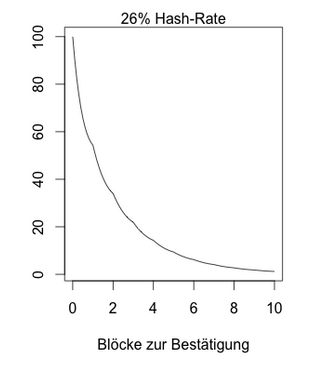
\includegraphics[scale=0.75]{26Prozent.PNG}%
\caption{Veranschaulichung zeigt wie unwahrscheinlich es wird, je weiter man zur�ckliegt (Quelle https://www.btc-echo.de/tutorial/bitcoin-51-attacke/)}%
\label{fig:26prozent}%
\end{figure}

Langfristig kann die Hauptkette nur ersetzt werden, wenn �ber 50\% der Hash-Rate dem Angreifer zur Verf�gung stehen.
\begin{figure}[h]%
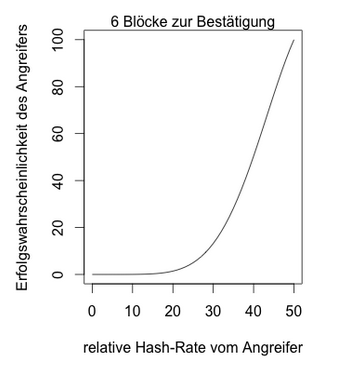
\includegraphics[scale=0.75]{51Prozent.PNG}%
\caption{Zeigt wie hoch die Wahrscheinlichkeit ist, sechs Bl�cke hintereinander zu generieren (Quelle https://www.btc-echo.de/tutorial/bitcoin-51-attacke/)}%
\label{fig:51prozent}%
\end{figure}

Satoshi Nakamoto f�hrt folgende Formel zur Berechnung der Wahrscheinlichkeit an, dass ein Angreifer die Blockchain einholen kann aus \emph{z} Bl�cken im R�ckstand. Der zeitliche Rahmen ist unbegrenzt.

$ p = $ Wahrscheinlichkeit, dass ein ehrlicher Node den n�chsten Block erstellt\\
$ q = $ Wahrscheinlichkeit, dass der Angreifer den n�chsten Block erstellt\\
$ q_{z} = $ Wahrscheinlichkeit, dass der Angreifer die ehrliche Blockchain �berhohlt\\

$ q_{z} = 1 \quad if\ p\leq q \\
q_{z} = $ ( $ \frac{p}{q} $ ) $^{z} \quad if\ p > q $

Es geht hervor, dass die Chancen des Angreifers die Hauptkette zu �berhohlen bei unter 50\% Hash-Rate exponentiell schwinden.

Diese Angriffsfl�che er�ffnet sich aufgrund der dezentralen Architektur von Blockchain und ist ein integraler Bestandteil eines, auf Konsens beruhenden, Systems.

\subsection{Anreiz zur Ehrlichkeit}
Durch die Entlohnung in Form von Bitcoins durch das Minen und durch die Transaktionsgeb�hren wird an Anreiz geschaffen, das Bitcoin-Netzwerk nicht zu manipulieren. Eine Kette mit ung�ltigen Bl�cken w�rde auch nicht von ehrlichen Minern angenommen werden. Daher wird erhofft (Nakamoto whitepaper referenz), dass die Belohnung und das Eigeninteresse an der Integrit�t von Bitcoin ausreicht um Angreifer abzuwehren.

\subsection{Quantenprozessorresistenz}
Mit der Einf�hrung leistungsstarker Quantenprozessoren die darauf ausgelegt sind, kryptographische Algorithmen zu entschl�sseln k�nnten Algorithmen wie, unter anderem, ECDSA unsicher werden. Auch die starke Leistung von Quantencomputern er�ffnet eine neue Angriffsfl�che unter dem Aspekt, dass der Anteil von �ber der H�lfte der Gesamtleistung des Miner-Netzwerkes dem Nutzer langfristig eine l�ngere Blockchain gew�hren kann, auf dieses Problem wird in Kapitel \ref{bitcoin:angriffsszenarios} eingegangen.

Die genutzten kryptographischen Algorithmen sind nicht bewiesen, dass sie Quantenprozessoren standhalten k�nnten. Indes ist das Bitcoin-Netzwerk durch ihre Architektur und Nutzung nicht gegen Quantencomputern gesch�tzt. Aber komplett ungesch�tzt bleibt die Technologie nicht.

Auch wenn der ECDSA mit einem entsprechenden Algorithmus gel�st werden sollte, oder durch Quantenprozessoren in anderer Hinsicht unsicher werden sollte, wird durch das hashen des �ffentlichen Schl�ssels genau dieser verschleiert. Er kommt nur zum Vorschein, wenn von dieser Adresse eine Zahlung ausgeht, aufgrund der Signierung. Wenn nun von da an ein neues Schl�sselpaar generiert und genutzt wird, sollten die Bitcoins an der eigenen Adresse sicher sein.

\section{IOTA}
IOTA nutzt im Gegensatz zu Bitcoin keine Blockchain-Technologie, sondern setzt auf ein sogenanntes Tangle, welches wiederum auf einem mathematischem Konzept basiert, welches sich Directed-Acyclic-Graph (DAG) nennt (siehe zu Tangle Grundlagen \ref{grundlagen:tangle} auf Seite \pageref{grundlagen:tangle}). Dieses Konzept unterscheidet sich grunds�tzlich von Blockchain und weist unter diesem Aspekt andere Sicherheitsrisiken auf. Im folgenden sollen diese beschrieben werden.

\subsection{Konto Sicherheit}
Auch bei IOTA besteht das Konto aus einem digitalen Schl�ssel, dem Seed. Dieser Seed sollte nur dem Eigent�mer verf�gbar gemacht werden, da jede Person mit diesem Seed, �ber die zugeordneten IOTAs verf�gen kann. F�r einen optimalen Schutz vor digitalem Diebstahl nur lokal (ohne Internetzugang) erstellt und gespeichert werden. Wenn diese allgemeinen Sicherheitsvorschl�ge eingehalten werden, besteht hier noch kein nennenswertes Risiko.

Ein Seed besteht aus 81 Trytes (siehe zu Trytes Grundlagen \ref{grundlagen:tritsundtrytes} auf Seite \pageref{grundlagen:tritsundtrytes}). Ein Tryte enth�lt drei Trits und kann folglich 27 ganze Zahlen darstellen. Daraus ergeben sich $ 27^{81} \approx 8,72 \times 10^{115} $ verschiedene Kombinationsm�glichkeiten. Das hei�t, die Wahrscheinlichkeit, dass eine andere Instanz denselben Seed generiert wie der Eigent�mer ist $ 1 : 8,72 \times 10^{115} $, damit ist die Anzahl der Kombinationsm�glichkeiten deutlich h�her als die Anzahl der Atome im bekannten Universum.\\

Durch das One-Time-Winternitz hashing (hier referenz einf�gen zu entweder Grundlagen oder Funktion) ist eine Adresse f�r ausgehende Zahlungen nur einmal zu benutzen, da ein Teil des privaten Schl�ssels bekannt wird, sollte die Adresse mehr als einmal genutzt werden, so wird zu viel des privaten Schl�ssels �ffentlich gemacht und eine Entschl�sselung wird zunehmend einfacher. Ist der private Schl�ssel vollst�ndig enth�llt, kann der Angreifer auf die IOTAs zugreifen die auf der Adresse hinterlegt sind.

Hierdurch er�ffnet sich ein Risiko, welches der Nutzer von IOTA selbst entgegnen muss, wenn er nicht das offizielle IOTA-Wallet Programm nutzt um Transaktionen zu erstellen. Hierzu muss angemerkt werden, dass durch die Kompromittierung des privaten Schl�ssels nicht der Seed oder alle anderen Adressen gef�hrdet sind.

\subsection{Anonymit�t}
Es ist wichtig zu betrachten, wie Anonym die Identit�t im Tangle-Netzwerk ist. Zum einen was einige Nutzer �ber andere Nutzer wissen k�nnen und zum anderen was in einer Transaktion �ber die Identit�t preisgegeben wird.

Vorerst muss notiert werden, dass Anonymit�t keine Priorit�t in der Entwicklung von IOTA gewesen ist und auch nicht prim�r f�r diesen Zweck entwickelt worden ist. (Quelle bitte angeben)
- bezahlen mit bitcoin, was wird �ber die identit�t revealed\\

Um eine Transaktion zu veranlassen wird ein Paar aus privatem und �ffentlichem Schl�ssel ben�tigt, welche aus dem Seed und einem Adressindex generiert werden. Der �ffentliche Schl�ssel dient hierbei als Adresse die man an seinen Transaktionspartner senden kann. Der private Schl�ssel sollte verborgen bleiben, denn jener Schl�ssel wird genutzt um die Inputs eines Bundles zu signieren. Damit wird bewiesen, dass der Ersteller der Transaktion den privaten Schl�ssel zu der Adresse besitzt und folglich der Eigent�mer ist.

\subsection{Validit�t einer Transaktion}
Eine Transaktion wird von anderen Nodes validiert. Typischerweise geschieht das wenn ein Nutzer eine Transaktion in das Tangle publizieren will. Daf�r muss der Nutzer zwei Transaktionen validieren. Bei diesen Transaktionen handelt es sich um "`Tips"', die noch nicht referenziert sind. Das Transaktionsobjekt muss die Tips als "`branch"'- und "`trunkTransaction"' referenzieren und �berpr�fen.

Das Objekt wird auf Syntax und G�ltigkeit gepr�ft. Daf�r wird der Transaction-Hash abgeglichen und die Signierung �berpr�ft. 

- wie wird eine einzelne transaktion verifiziert, wie wird bestimmt dass sie g�ltig ist\\
- wann ist eine transaktion verifiziert\\

\subsection{Angriffsszenarien}
Die Tangle erm�glicht durch ihre DAG spezifische Arten von Attacken die im weiteren Fortgang erl�utert werden sollen. Durch die Darstellung der m�glichen Angriffe, werden weitere Sicherheitsmechanismen veranschaulicht.

\subsubsection{34\%-Attacke}
Ein b�swilliger Nutzer k�nnte mit mehr als 34\% der Gesamtrechenleistung im Tangle-Netzwerk einen Angriff starten indem er falsche Transaktionen mit vielen anderen selbst initiierten Transaktionen verifiziert und damit im DAG einen Strang erzeugt der falsche Informationen �ber die verf�gbaren IOTAs enth�lt.

Dem entgegenwirken soll der, von der IOTA-Foundation bereitgestellte, Coordinator. Dieser ist ein Node, der eigenst�ndig Transaktionen erstellt, die als Meilenstein (Milestone) gelten. Der Milestone dient als Beweis, dass die vorherigen Transaktionen korrekt sind. Jede Transaktion muss diese Coordinators indirekt oder direkt referenzieren.

Diese Coordinators bieten jedoch eine neue Angriffsfl�che. Dabei geht es um das derzeit nicht vollkommen dezentrale System der Tangle bei IOTA. IOTA l�st also noch nicht das Problem, ohne dritte Instanz Transaktionen vermitteln zu k�nnen. Laut IOTA-Foundation sollen die Coordinators ihren Dienst einstellen, sobald das Tangle Netzwerk ausreichend gro� ist, um 34\%-Attacken durch eine zu hohe Anforderung an Rechenleistung abwehren zu k�nnen.

\subsubsection{Parasiten-Kette}

- wie sch�tzt sich das Bitcoin netzwerk vor Angriffen\\
- welche angriffsszenarios sind denkbar\\
- was kann dagegen getan werden\\

\subsection{Quantenprozessorresistenz}
Bei der Frage nach Zukunftssicherheit bei IOTA geht es auch um die Resistenz vor Quantenprozessoren. Genauer soll betrachtet werden, ob sich die Fertigstellung von diesen leistungsstarken Prozessoren auf die Sicherheit und Best�ndigkeit von IOTAs auswirkt.

Hierbei ist es n�tig, auf den Winternitz onetime hashing algorithmus zur�ckzugreifen um zu verstehen wie sich der Algorithmus auf Quantenresistenz auswirkt.

\section{Gegen�berstellung}
- Iota nennt sich nachfolger von blockchain, welche Sicherheits risiken wurden dort gel�st und welche sind neu aufgekommen

[Tabelle mit kriterien und vergleichen]

\section{Ergebnis}
Alles in allem, sind diese kryptos sicher? Auch im Bezug auf zukunftssicherheit
\chapter{Programmierbarkeit}
In diesem Abschnitt folgt eine Beschreibung der Programmierschnittstellen bei Bitcoin und IOTA. Dies ist relevant da gegebene Schnittstellen und Ressourcen f�r Programmierer die Einsetzbarkeit erh�hen. Wenn Entwickler auf den vorhandenen Code aufbauen und erweitern k�nnen, k�nnen die 
Eine aussage �ber die zuk�nftigen einsatzm�glichkeiten

\section{Bitcoin}
Der Code f�r Bitcoin ist Open-Source und damit frei zug�nglich
Ja was gibts bei bitcoin so keine ahnung

\section{IOTA}
Iota erlaubt 0 vlaue transactions f�r meta daten zb json datein (nutzen hiervon f�r alltag umstritten wegen stormverbrauch), das erlaubt also quasi vershcicken von daten in der tangle
Dadurch erschlie�t sich ein weiterer Anwendungsbereich. Diese Funktion erlaubt eine n�tzliche Anwendung f�r das "`Internet der Dinge"' (internet of things \ref{} auf seite \pageref{}
\chapter{Nutzen}
\section{IOTA}
IOTA wurde in erster Linie f�r das "`Internet of Things"' entworfen und soll Transaktionen und Kommunikationen sowohl zwischen Menschen als auch zwischen Ger�tschaften erm�glichen. Die Vision der IOTA-Foundation beschreibt die Tangle und das dazugeh�rige Distributed Ledger Protokoll, als eine einheitliche �bereinstimmung der Richtigkeit von Daten. Dieses Prinzip wird �ber kryptographische Hash Verfahren erreicht. Des weiteren m�chte IOTA eine L�sung f�r den wachsenden globalen Datentransfer liefern, indem das Server - Client Modell durch eine dezentrale L�sung ersetzt wird. Im Folgenden wird die Kommunikation in der Tangle durch die Verwendung von "`Masked Authenticated Message"' (kurz MAM) im Detail beleuchtet.

\subsection{MAM}
MAM steht f�r "`Masked Authenticated Message"' und ist die L�sung f�r das Kommunizieren innerhalb der Blockchain. Es ist m�glich durch eine wertlose Transaktion eine Nachricht zu verschicken. Sollen jedoch mehrere Nachrichten versendet werden, bspw. soll die Temperatur eines Motors alle 15 Minuten aktualisiert werden, treten einige Probleme auf. Der Versender kann die Nachricht zwar immer an die gleiche Adresse versenden, aber jeder andere IOTA Benutzer auch. Bei einem m�glichen b�swilligen Angriff k�nnten die validen Nachrichten nicht von den b�swilligen unterschieden werden.

MAM basiert auf Kan�len die ein interessierter H�rer "`abonnieren"' kann. Es werden Transaktionen generiert die jeweils den Index des Branches, die Geschwister - Knoten des Merkle Trees, die Adresse der n�chsten Generation und die Nachricht als Hash enthalten. MAM�s verweisen immer auf die n�chste Generation, aber nie auf die vergangene Generation oder den Genesis.

\paragraph{Verschl�sselung}
Abh�ngig davon in welchem Modus die Daten publiziert sind, ben�tigt der H�rer entweder ausschlie�lich den "`root"' oder zus�tzlich einen  �sideKey� um die Daten zu entschl�sseln. In dem Modus "`public"' kann der Inhalt durch den "`root"' entschl�sselt werden. Sollte der Modus "`restricted"' sein, ist es zwar m�glich die MAM mit Hilfe des "`root"' in der Tangle zu finden, um die Daten jedoch zu entschl�sseln wird ein "`sideKey"' ben�tigt. Derjenige, der die Daten publiziert, kann dementsprechend entscheiden, wer die Daten einsehen kann.

\paragraph{Signatur}
Ein b�swilliger H�rer, der von einem Kanal den "`root"' und den "`sideKey"' erh�lt, darf nicht die M�glichkeit haben, dank dieser beiden Daten, den Kanal f�r sich zu beanspruchen um zuk�nftig Beitr�ge in diesem zu verfassen. Der Kanal ben�tigt eine Signatur. Diese wird nach dem "`Merkle tree based signature scheme"' erreicht. Eine Generation ist aufgebaut wie ein Merkle Tree. Die Bl�tter sind private Schl�ssel. Diese Schl�ssel werden verwendet um IOTA-Adressen zu generieren. Adressen werden jeweils paarweise miteinander gehasht. Das paarweise Hashen der Ergebnisse wird solange fortgef�hrt, bis der root Hash erreicht ist. Es k�nnen beliebig viele Generationen erstellt werden. Der H�rer nutzt die Adresse der MAM und hasht diesen mit dem ersten, in der MAM angegebenen Geschwister Hash. Das Ergebnis wird mit dem n�chsten Geschwister Hash zusammengef�hrt. Dieser Vorgang wiederholt sich, bis das letzte Paar zu dem sogenannten "`temp\_root"' zusammengef�hrt wurde. Sollte der "`temp\_root"' identisch mit dem root der MAM sein, ist die Nachricht authentisch.\footnote{Daten bezogen von: https://medium.com/coinmonks/iota-mam-eloquently-explained-d7505863b413}

\section{Bitcoin}
Bitcoin wurde als eine kryptographische W�hrung implementiert, die erstmalig das anonyme, dezentrale Bezahlen erm�glicht. Der Nutzen wird dadurch deutlich, dass die Bezahlvorg�nge unabh�ngig von Gesetzen oder Richtlinien durchgesetzt werden k�nnen. Einer Transaktion im Bitcoin Netzwerk ist nicht ersichtlich, welche Ware eingekauft wurde und welche Person f�r die Bezahlung zust�ndig ist. Das Netzwerk ist g�nzlich unabh�ngig von der Kontrolle einer zentralen Partei. Jeder Bezahlvorgang ist in der Blockchain dokumentiert und f�r jedermann einsehbar.

Diese Eigenschaften sorgen daf�r, dass das Vertrauen nicht mehr auf einer zentralen Vertrauenspartei basiert, sondern das Netzwerk daf�r einsteht. Jede je get�tigte Transaktion kann zu einem beliebigen Zeitpunkt in der Zukunft r�ckwirkend verifiziert werden, ohne dass Rechte Dritter verletzt werden.

Die Blockchain hinter Bitcoin setzt den Grundstein f�r einen sicheren Umgang mit finanziellen und kommerziellen G�tern. So k�nnte die Echtheit von sensiblen Dokumenten durch deren digitalen Fingerabdruck unwiderruflich in der Blockchain abgespeichert werden. Ein Mietvertrag, dessen Mietkosten monatlich zu begleichen sind, k�nnten in Form eines "`Smart Contracts"' durch die Blockchain auf Richtigkeit �berpr�ft und ausgef�hrt werden.~\cite{je:useBitcoin}

\chapter{Ergebnis}
\chapter{Zusammenfassung}
\chapter{Realisierung des Prototypen}
Um eine bessere Aussage �ber die Zukunftstauglichkeit von Distributed Ledger Technologien zu gewinnen, wird gemeinsam mit der IOTA Technologie ein Anwendungsfall prototypisch implementiert. Bei diesem Anwendungsfall handelt es sich um eine Tankstelle an der ein Auto m�glichst autonom den Tankvorgang startet und im Anschluss den anfallenden Betrag mit der Kryptow�hrung IOTA begleicht. Die kommende Ausf�hrung befasst sich mit der Implementation eines Prototypen.

Aus dem analytischen Teil folgt, dass zwischen Bitcoin und IOTA deutliche Unterschiede herrschen. F�r die Auswahl einer Distributed Ledger Technologie wurden Faktoren wie Best�tigungszeit und Transaktionsgeb�hren miteinbezogen. Ein weiterer Grund f�r die Auswahl einer Technologie war die Dokumentation ihrer Bibliotheken.

Aufgrund einer vorhandenen Dokumentation, schnellen Verifizierungen von Transaktionen und das fehlen einer Geb�hr wurde IOTA f�r die Implementierung ausgew�hlt.

\chapter{Fahrzeug - Client}
Das Programm soll f�r einen realit�tsnahen Anwendungsfall auf einem relativ leistungsschwachen System arbeiten k�nnen. Daher liegt es nahe f�r die Programmierung des Programmierteils, der f�r das Tanken und Bezahlen mit IOTAs zust�ndig ist, einen Raspberry Pi anzusteuern.

Der Raspberry Pi soll in dieser prototypischen Umsetzung die Steuereinheit eines zuk�nftigen Autos ersetzen. Es soll mittels zwei Kn�pfen bedienbar sein, die die Steuerelemente in der Armatur des Autos darstellen sollen.

Da der Anspruch an starke Rechenleistung in einem Auto nicht zu hoch sein sollte (um zum Beispiel Kosten zu minimieren) ist es sinnvoll, keinen IOTA Full-Node zu betrieben, sondern nur einen Light-Node, der die Arbeit an einen Full-Node delegiert. Die Limitation der Hardware-Ressourcen ist ein Grund f�r die Umsetzung auf einem Raspberry Pi.

Die Anforderungen an das Smartauto sind wie folgt:
\begin{itemize}
	\item Der Nutzer muss vor dem dem Tankvorgang �ber die Tankstelle informiert werden
	\item Der Nutzer soll mit einem Knopfdruck tanken k�nnen
	\item Der Nutzer soll mit einem Knopfdruck bezahlen k�nnen, ohne das weitere Eingaben notwendig sind
	\item Die Transaktion muss schnell von der Tankstelle validiert werden
\end{itemize}
An diese Anforderungen orientiert sich die folgende Umsetzung.


\section{Aufbau}
Unter diesem Aspekt wird der Aufbau und die Einrichtung der einzelnen Komponenten beschrieben die f�r die Umsetzung n�tig sind.

\subsection{Vorbedingungen}
Unter diesem Aspekt werden die Voraussetzungen f�r die Umsetzung der clientseitigen Tankanwendung beschrieben. Diese Vorbedingungen wurden genutzt um den Raspberry Pi so einzurichten und zu konfigurieren, damit das Ger�t die Anforderungen an das Programm erf�llen kann.

Um die prototypische Anwendung umsetzen zu k�nnen, werden folgende Komponenten genutzt:

\subsubsection{Raspberry Pi 3 Model B}
Auf dem Raspberry Pi wird die Anwendung ausgef�hrt, Daten des Benutzers verarbeitet und Anfragen auf Webservices vollzogen. Auch die Transaktionen von IOTAs sollen mithilfe des CPUs erstellt werden.

\subsubsection{Steckbrett}
Das Steckbrett dient der Verbindung von Bedienelementen mit den GPIO-Pins des Raspberry Pis. Die Kn�pfe f�r die Bedienung der Tank-Anwendung werden auf diesem befestigt und mit den GPIO-Pins elektronisch verbunden.

\subsubsection{Micro SD Karte}
Diese Speicherkarte wird f�r den Raspberry Pi gebraucht. Auf dieser befindet sich das Betriebssystem mit dem der Raspberry Pi erst genutzt werden kann. Auch das Programm und sonstige Benutzerdaten werden auf dieser Speicherkarte gespeichert.

\subsubsection{Micro USB Netzteil 5,1 Volt 3,1 Ampere}
Der Raspberry Pi muss mittels eines Micro USB Eingangs mit Strom versorgt werden. Das Netzteil sollte eine Ausgangsspannung von mindestens 5,1 Volt aufweisen und es werden mindestens 2,5 Ampere empfohlen\footnote{Nach https://www.raspberrypi.org/documentation/hardware/raspberrypi/power/README.md}.

\subsubsection{5x Weiblich-M�nnlich Kabel, 2x M�nnlich-M�nnlich Kabel}
Verbindungskabel f�r das Steckbrett um elektronische Komponenten miteinander zu Verbinden.

\subsubsection{2x Taster, 1x Rote LED}
Elektronische Komponenten um dem Benutzer der Anwendung Bedienelemente zur Verf�gung zu stellen. Die LED dient f�r ein visuelles Feedback.

\subsubsection{Widerst�nde 1x 330 Ohm, 2x 10.000 Ohm, 2x 1.000 Ohm}
Die Widerst�nde sind f�r den kontrollierten Stromfluss unentbehrlich und sie verhindern, dass die Komponenten durch zu hohen Stromfluss besch�digt werden.

\subsection{Einrichtung}
Um den Raspberry Pi so einzurichten, dass es m�glich ist, Anwendungen zu programmieren und zu testen, sollte dieser mittels eines HDMI-Kabels an einen Monitor angeschlossen werden. Weiterhin sollten Peripherieger�te wie Tastatur und Maus �ber die USB-Ausg�nge angeschlossen werden um sich durch die Bedienoberfl�che navigieren zu k�nnen. Doch damit das Ger�t vollst�ndig bedienbar wird, muss es mit einem Betriebssystem ausgestattet sein. Aufgrund von offiziellem Support seitens der Raspberry Pi Foundation [26](Quelle) wurde das Raspbian Betriebssystem f�r die Umsetzung ausgew�hlt. Bei Raspbian handelt es sich um ein, auf Linux basierendes Betriebssystem, welches von der Raspberry Pi Foundation ver�ffentlicht wurde.

Das Raspbian Betriebssystem muss auf die Micro SD Karte geladen werden, damit es f�r den Raspberry Pi zur Verf�gung steht. In folgenden Schritten wurde die Speicherkarte mit Raspbian beschrieben:
\begin{enumerate}
	\item Download von Raspbian (https://www.raspberrypi.org/downloads/)
	\item Gegebenenfalls .zip/.rar entpacken
	\item Speicherkarte in ein Kartenleseger�t stecken
	\item Mithilfe eines Brennprogramms die Imagedatei auf die Speicherkarte brennen (flashen)
\end{enumerate}

Die Speicherkarte ist nun formatiert und mit Raspbian ausgestattet, sie kann nun aus dem Kartenleseger�t genommen werden und in den Raspberry Pi gesteckt werden.

Nachdem das Ger�t zum ersten Mal gestartet wird, muss das Betriebssystem einmalig eingerichtet werden. Wenn dies geschehen ist, sollte man jegliche Software-Pakete in Raspbian updaten um m�gliche Fehler vorzubeugen. Dies kann mit folgenden Befehlen in dem Terminal des Betriebssystems vollzogen werden:

\begin{lstlisting}[language=bash]
> sudo apt-get update
> sudo apt-get dist-upgrade
\end{lstlisting}

\subsubsection{Steckbrett und GPIO-Pins}
Die Taster und LEDs m�ssen elektrisch mit den GPIO-Pins verbunden werden, um von dem Raspberry Pi angesprochen werden zu k�nnen. Die Taster stellen Kn�pfe auf der Armatur des Autos dar. Die LED dient daf�r, ein visuelles Feedback zu geben, zum Beispiel im Bezug auf die Tank-Anwendung ob nun getankt werden kann.

Daf�r ist es n�tzlich, mit dem Pin-Layout des Raspberry Pis vertraut zu sein. Mit dem Terminal-Befehl

\begin{lstlisting}[language=bash]
> pinout
\end{lstlisting}

ist es m�glich einen �berblick �ber das Layout des Raspberry Pis zu erhalten. Auch die Benennung der einzelnen Pins ist aufgef�hrt.

\begin{figure}[H]%
\centering
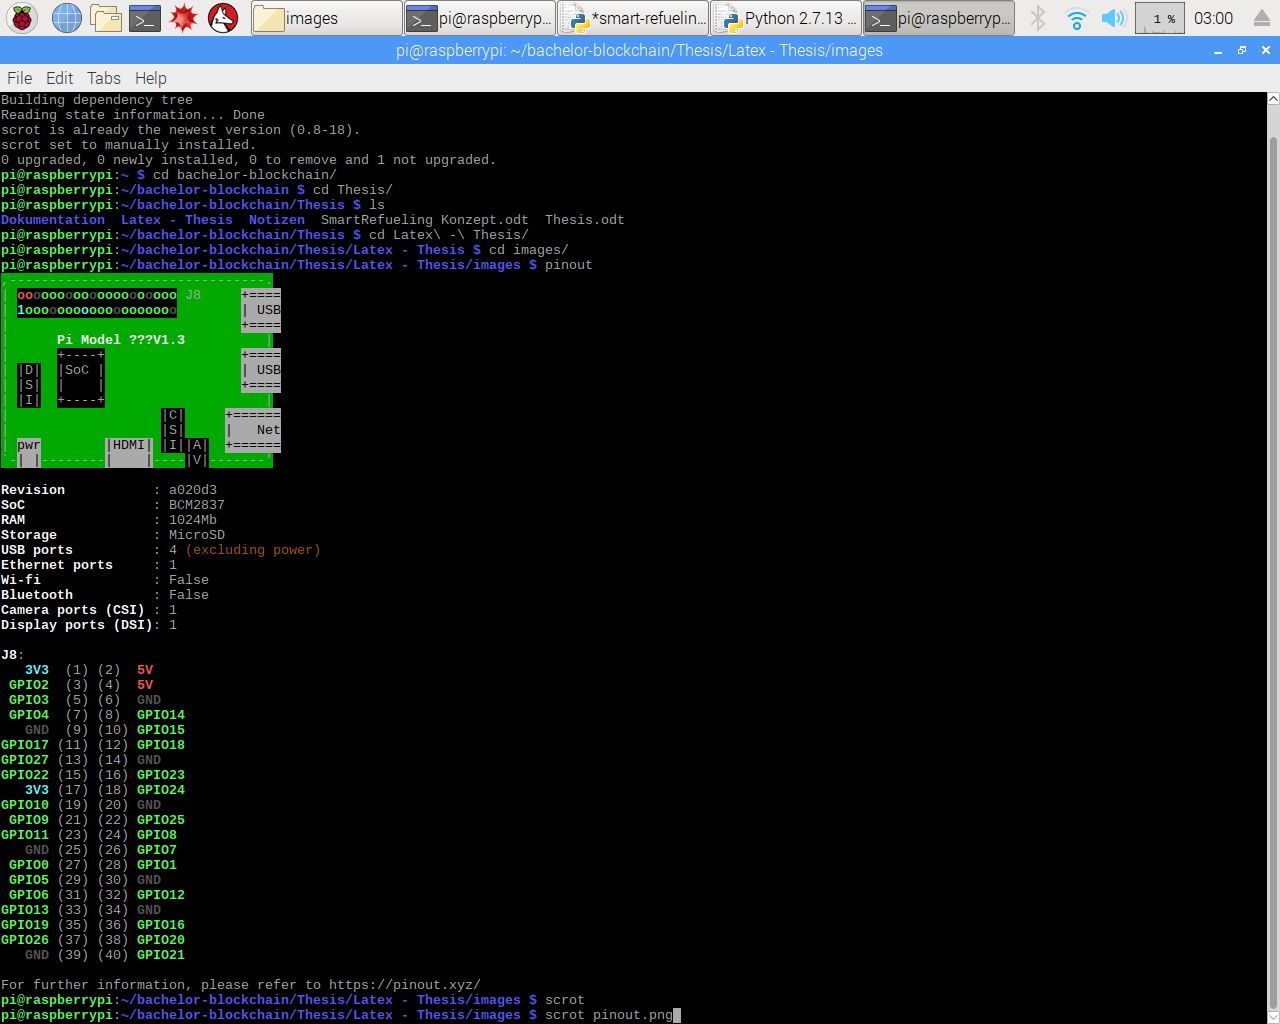
\includegraphics[scale=0.6]{pinout.png}%
\caption{Pinout-Ausgabe}
\end{figure}

Die Komponenten m�ssen in das Steckbrett gesteckt werden, sodass sie erreichbar bleiben, um sie zu verkabeln und zugleich nutzen zu k�nnen. F�r eine optimale �bersicht wurden die Komponenten mittig platziert.

F�r die Umsetzung m�ssen diese Komponenten f�r den Nutzer interagierbar sein, dazu werden sie mit zuf�lligen, freien GPIO-Pins verbunden.

\begin{table}[H]%
\centering
\begin{tabular}{l|l}
Komponente & GPIO-Pin\\
\hline
Button 1 & 11\\
Button 2 & 22\\
LED & 10
\end{tabular}
\caption{Korrespondenz der Buttons mit den GPIO-Pins}
\label{buttonlayout}
\end{table}

\subsubsection{PyOTA}
Bei PyOTA handelt es sich um eine Python-Bibliothek f�r IOTA. Sie implementiert die API und unterst�tzt Funktionalit�ten um eine Transaktion eigenst�ndig erstellen zu k�nnen\footnote{siehe dazu https://pyota.readthedocs.io/en/latest/}.

Um die Bibliothek f�r die Umsetzung zur Verf�gung zu stellen kann sie �ber das Paketverwaltungsprogramm f�r die Umgebung installiert werden.
\begin{lstlisting}[language=bash]
> pip install pyota
\end{lstlisting}

Eine wichtige Abh�ngigkeit (Dependancy) von PyOTA ist die Cryptography-Bibliothek. Diese wird nicht automatisch heruntergeladen und installiert, sondern dies muss manuell geschehen\footnote{mehr Informationen dazu https://cryptography.io/en/latest/installation/}.

Weiterhin muss angemerkt werden, das bei Raspbian kein System-Pfad zu den zus�tzlich installierten Paketen (per pip install) f�r Python2.7 gibt. Demzufolge muss der Pfad vor jedem Programmstart in das Suchverzeichnis hinzugef�gt werden. Dies geschieht mit folgendem Code:
\begin{lstlisting}[language=Python]
import sys
sys.path.append("/home/pi/.local/lib/python2.7/site-packages")  #path muss erweitert werden damit PyOta librarys gefunden werden k�nnen
\end{lstlisting}

\subsection{Ergebnis der Vorbereitung}
Nachdem alle Vorbedingungen erf�llt sind, ist der Raspberry Pi einsatzbereit um ein Programm zu erstellen und auszuf�hren, welches auf Benutzereingaben an Kn�pfen horcht, visuelles Feedback gibt und mit der PyOta-Bibliothek arbeitet.

\section{Umsetzung}
In diesem Abschnitt sollen die ausgew�hlten Programmierans�tze gezeigt und besprochen werden. Es soll ein �berblick �ber die verwendeten Methoden geschaffen werden. Bei mehreren m�glichen Methoden soll dar�ber hinaus deutlich werden, warum die entsprechende Methode gew�hlt wurde.

\subsection{GPIO-Pins}
Auf dem Raspberry Pi m�ssen die GPIO-Pins vorkonfiguriert werden um danach einzelne Pins als Inputs oder Outputs setzen zu k�nnen. Die Funktionalit�t wird der vorinstallierten RPi.GPIO-Bibliothek entnommen. Sie wird zur Abk�rzung fortan mit "`GPIO"' referenziert.
\begin{lstlisting}[language=Python]
import RPi.GPIO as GPIO     #importiere GPIO-Bibliothek f�r Ein-/Ausgaben von Inputs und Outputs (Buttons/LEDs)
\end{lstlisting}

Zum Ansprechen der Pins muss bestimmt werden, welche Pins mit welcher Nummer korrespondieren. Zum Beispiel hat Pin 12 eine Zweideutigkeit in dem Sinne, dass er zum einen Pin 12 bei einer, numerisch sortierten Aneinanderreihung, der zw�lfte Pin des Panels ist. Zum anderen kann sich Pin 12 auch auf den Namen des Pins beziehen, in diesem Beispiel "`GPIO12"', welcher sich nicht an einer numerischen Anordnung befindet.

Daher muss der Modus des Boards gesetzt werden mit folgender Code Zeile.
\begin{lstlisting}[language=Python]
GPIO.setmode(GPIO.BCM)
\end{lstlisting}
GPIO.BCM bezieht sich auf den Broadcom SOC (system on chip) Kanal, der angesprochen wird. Die Auswahl von dieser Variante hat keine Vor- oder Nachteile f�r das Projekt und wurde arbitr�r ausgew�hlt.

Nachdem der Modus eingestellt wurde kann nun die Datenrichtung der Pins bestimmt werden. Daf�r wird der Pin als Input oder als Output gesetzt.
\begin{lstlisting}[language=Python]
BUTTON1 = 11
BUTTON2 = 22
LED = 10

GPIO.setup(BUTTON1, GPIO.IN)
GPIO.setup(BUTTON2, GPIO.IN)
GPIO.setup(LED, GPIO.OUT, initial = False)
\end{lstlisting}

Nun sind die einzelnen Pins manipulierbar, bzw. auslesbar. Je nachdem ob man einen Output-Pin setzten m�chte oder einen Input-Pin auslesen m�chte, sind verschiedene Funktionen verwendbar.

Zum Auslesen ob ein Knopf gedr�ckt wurde bietet sich die folgende einfache Implementierung an. Das Programm wartet solange, bis der Knopf gedr�ckt und losgelassen wurde.
\begin{lstlisting}[language=Python]
def wait_for_button_click(button):
    while not GPIO.input(button):
        pass
    while GPIO.input(button):
        pass
\end{lstlisting}
Wobei der Parameter 'button' die Pin-Nummer referenziert.\\
Es bieten sich auch andere, effizientere Methoden an, jedoch ist diese Implementierung f�r den Prototypen ausreichend.

Um einen Output wie zum Beispiel die LED zu setzen, ben�tigen wir diese Code-Zeile:
\begin{lstlisting}[language=Python]
GPIO.output(LED, True)
\end{lstlisting}

\subsection{IOTA Einrichtung}
Unter der Einrichtung von IOTA ist zu verstehen, die IOTA-Bibliothek so zu utilisieren, dass mit der API eine Transaktion in das Tangle-Netzwerk ver�ffentlicht werden kann. F�r so eine Funktionalit�t bietet sich das Iota-Objekt an. Dieses wird dank des iota-Moduls bereitgestellt.
\begin{lstlisting}[language=Python]
from iota import Iota
\end{lstlisting}

Damit nun das Iota Objekt initialisiert werden kann, braucht es zwei Argumente. Den Seed, und eine Adresse zu einer Full-Node.

\paragraph{Seed} Der Seed "`DSPOAXMVSC99IUIVJXTIBZFATVFKTCLLJYOLAGSMFJGFXAWEB9GNTQWEDVRYHKIOQF9T9IZY9IVPKTSZK"' wurde aus einer zuf�lligen Kombination der Gro�buchstaben 'A-Z' und der Nummer 9 eigenh�ndig generiert und wird f�r den Prototypen genutzt. Im Programmcode ist der Seed hinterlegt, dies k�nnte bei einer realistischen Umgebung zu Sicherheitsrisiken f�hren, f�r die prototypische Umsetzung gen�gt es.

\paragraph{Full-Node} Aus einer Liste im Internet\footnote{siehe https://iotasalad.org/nodes}, in der einige Full-Nodes aufgelistet sind, wurde die folgende Adresse beliebig ausgesucht: https://potato.iotasalad.org:14265. Der Full-Node �bernimmt die Arbeit die erstellte Transaktion in das Tangle zu ver�ffentlichen, da der Raspberry Pi zu leistungsschwach ist um den Proof-Of-Work zeiteffizient zu �bernehmen.

Aus den gegebenen Parametern kann das Iota-Objekt erstellt werden.
\begin{lstlisting}[language=Python]
seed = "DSPOAXMVSC99IUIVJXTIBZFATVFKTCLLJYOLAGSMFJGFXAWEB9GNTQWEDVRYHKIOQF9T9IZY9IVPKTSZK"  
fullnode_url = "https://potato.iotasalad.org:14265"
api = Iota(fullnode_url, seed)
\end{lstlisting}

Es ist nun m�glich, grundlegende Funktionen wie Adressgenerierung nutzen zu k�nnen.

\subsection{IOTA Transaktion}
Um eine Transaktion zu erstellen werden f�r diese Implementierung die Klassen ProposedTransaction, ProposedBundle, Address, Tag und TryteString zus�tzlich zu Iota von dem iota-Modul genutzt.
\begin{lstlisting}[language=Python]
from iota import Iota, ProposedTransaction, ProposedBundle, Address, Tag, TryteString
\end{lstlisting}

Vorerst muss ein "`Vorabtransaktions"'-Objekt erstellt werden mit Adresse, Wert, Tag und Message.
\begin{lstlisting}[language=Python]
proposedTrx = ProposedTransaction(
    address = Address(reciever_address),
    value = 0,
    tag = Tag("BACHELORTEST"),
    message = TryteString.from_string("This is a test transaction")
)
proposedBundle = ProposedBundle([proposedTrx])
\end{lstlisting}
Das Transaktionsobjekt wird gef�llt mit der Empf�ngeradresse, dem Wert 0 (eine "`Meta Transaction"'), einem Tag welcher mithilfe des Tag-Objekts erstellt wird und einer beliebigen Nachricht, welche mithilfe von TryteString in Trits umgewandelt wird. Abschlie�end wird ein "`Vorabbundle"' erstellt, welches mit der Vorabtransaktion bef�llt wird.

Dieses Vorabbundle muss gepr�ft und signiert werden, daf�r wird es als Parameter an die vorher erstellte Iota-Instanz �bergeben. Der Aufruf gibt ein vorbereitetes Bundle zur�ck, welches mittels API-Aufruf an die Full-Node verschickt wird. Dort wird sie abschlie�end verarbeitet und in das Tangle-Netzwerk ver�ffentlicht.
\begin{lstlisting}[language=Python]
preparedBundle = api.prepare_transfer(proposedBundle)
publishedBundle = api.send_transfer(depth = 3, transfers = proposedBundle)
\end{lstlisting}

Die Hash des PublishedBundle-Objekts kann genutzt werden, um die Transaktion nachzuvollziehen\footnote{z.B auf https://iotasear.ch/}.

\subsection{Kommunikation mit Tankstelle}
Die Kommunikation mit der Tankstelle erfolgt �ber eine REST API. Dies ist vereinfacht betrachtet eine Schnittstelle auf die �ber HTTP zugegriffen werden kann. Hierf�r bietet sich das vorinstallierte requests-Modul an.
\begin{lstlisting}[language=Python]
import requests #importiere requests-Bibliothek um HTTP-Anfragen zu erstellen
\end{lstlisting}

Ein Beispiel eines Anwendungsfalles ist das Beenden des Tankvorgangs. Der Code hierf�r ist in einer Methode ausgelagert mit den Argumenten 'route' und 'carId'. Die 'route' ist die Schnittstelle die angesprochen werden soll, in diesem Beispiel "`endFueling"'. Die 'carId' ist eine von der Tankstelle zugewiesene Nummer. Das Beispiel verschickt eine Anfrage an den Server (die Tankstelle) mit einem Parameter, der Identifikationsnummer des Autos, und gibt die Antwort zur�ck.
\begin{lstlisting}[language=Python]
endFuelingData = call_api("endFueling", carId)

def call_api(route, carId):
		params = {
				"id": carId
		}
	response = requests.get(fueling_url + route, params)
return response.json()
\end{lstlisting}

\chapter{Fahrzeug - Client}
Das Programm soll f�r einen realit�tsnahen Anwendungsfall auf einem relativ leistungsschwachen System arbeiten k�nnen. Daher liegt es nahe f�r die Programmierung des Programmierteils, der f�r das Tanken und Bezahlen mit IOTAs zust�ndig ist, einen Raspberry Pi anzusteuern.

Der Raspberry Pi soll in dieser prototypischen Umsetzung die Steuereinheit eines zuk�nftigen Autos ersetzen. Es soll mittels zwei Kn�pfen bedienbar sein, die die Steuerelemente in der Armatur des Autos darstellen sollen.

Da der Anspruch an starke Rechenleistung in einem Auto nicht zu hoch sein sollte (um zum Beispiel Kosten zu minimieren) ist es sinnvoll, keinen IOTA Full-Node zu betrieben, sondern nur einen Light-Node, der die Arbeit an einen Full-Node delegiert. Die Limitation der Hardware-Ressourcen ist ein Grund f�r die Umsetzung auf einem Raspberry Pi.

Die Anforderungen an das Smartauto sind wie folgt:
\begin{itemize}
	\item Der Nutzer muss vor dem dem Tankvorgang �ber die Tankstelle informiert werden
	\item Der Nutzer soll mit einem Knopfdruck tanken k�nnen
	\item Der Nutzer soll mit einem Knopfdruck bezahlen k�nnen, ohne das weitere Eingaben notwendig sind
	\item Die Transaktion muss schnell von der Tankstelle validiert werden
\end{itemize}
An diese Anforderungen orientiert sich die folgende Umsetzung.


\section{Aufbau}
Unter diesem Aspekt wird der Aufbau und die Einrichtung der einzelnen Komponenten beschrieben die f�r die Umsetzung n�tig sind.

\subsection{Vorbedingungen}
Unter diesem Aspekt werden die Voraussetzungen f�r die Umsetzung der clientseitigen Tankanwendung beschrieben. Diese Vorbedingungen wurden genutzt um den Raspberry Pi so einzurichten und zu konfigurieren, damit das Ger�t die Anforderungen an das Programm erf�llen kann.

Um die prototypische Anwendung umsetzen zu k�nnen, werden folgende Komponenten genutzt:

\subsubsection{Raspberry Pi 3 Model B}
Auf dem Raspberry Pi wird die Anwendung ausgef�hrt, Daten des Benutzers verarbeitet und Anfragen auf Webservices vollzogen. Auch die Transaktionen von IOTAs sollen mithilfe des CPUs erstellt werden.

\subsubsection{Steckbrett}
Das Steckbrett dient der Verbindung von Bedienelementen mit den GPIO-Pins des Raspberry Pis. Die Kn�pfe f�r die Bedienung der Tank-Anwendung werden auf diesem befestigt und mit den GPIO-Pins elektronisch verbunden.

\subsubsection{Micro SD Karte}
Diese Speicherkarte wird f�r den Raspberry Pi gebraucht. Auf dieser befindet sich das Betriebssystem mit dem der Raspberry Pi erst genutzt werden kann. Auch das Programm und sonstige Benutzerdaten werden auf dieser Speicherkarte gespeichert.

\subsubsection{Micro USB Netzteil 5,1 Volt 3,1 Ampere}
Der Raspberry Pi muss mittels eines Micro USB Eingangs mit Strom versorgt werden. Das Netzteil sollte eine Ausgangsspannung von mindestens 5,1 Volt aufweisen und es werden mindestens 2,5 Ampere empfohlen\footnote{Nach https://www.raspberrypi.org/documentation/hardware/raspberrypi/power/README.md}.

\subsubsection{5x Weiblich-M�nnlich Kabel, 2x M�nnlich-M�nnlich Kabel}
Verbindungskabel f�r das Steckbrett um elektronische Komponenten miteinander zu Verbinden.

\subsubsection{2x Taster, 1x Rote LED}
Elektronische Komponenten um dem Benutzer der Anwendung Bedienelemente zur Verf�gung zu stellen. Die LED dient f�r ein visuelles Feedback.

\subsubsection{Widerst�nde 1x 330 Ohm, 2x 10.000 Ohm, 2x 1.000 Ohm}
Die Widerst�nde sind f�r den kontrollierten Stromfluss unentbehrlich und sie verhindern, dass die Komponenten durch zu hohen Stromfluss besch�digt werden.

\subsection{Einrichtung}
Um den Raspberry Pi so einzurichten, dass es m�glich ist, Anwendungen zu programmieren und zu testen, sollte dieser mittels eines HDMI-Kabels an einen Monitor angeschlossen werden. Weiterhin sollten Peripherieger�te wie Tastatur und Maus �ber die USB-Ausg�nge angeschlossen werden um sich durch die Bedienoberfl�che navigieren zu k�nnen. Doch damit das Ger�t vollst�ndig bedienbar wird, muss es mit einem Betriebssystem ausgestattet sein. Aufgrund von offiziellem Support seitens der Raspberry Pi Foundation [26](Quelle) wurde das Raspbian Betriebssystem f�r die Umsetzung ausgew�hlt. Bei Raspbian handelt es sich um ein, auf Linux basierendes Betriebssystem, welches von der Raspberry Pi Foundation ver�ffentlicht wurde.

Das Raspbian Betriebssystem muss auf die Micro SD Karte geladen werden, damit es f�r den Raspberry Pi zur Verf�gung steht. In folgenden Schritten wurde die Speicherkarte mit Raspbian beschrieben:
\begin{enumerate}
	\item Download von Raspbian (https://www.raspberrypi.org/downloads/)
	\item Gegebenenfalls .zip/.rar entpacken
	\item Speicherkarte in ein Kartenleseger�t stecken
	\item Mithilfe eines Brennprogramms die Imagedatei auf die Speicherkarte brennen (flashen)
\end{enumerate}

Die Speicherkarte ist nun formatiert und mit Raspbian ausgestattet, sie kann nun aus dem Kartenleseger�t genommen werden und in den Raspberry Pi gesteckt werden.

Nachdem das Ger�t zum ersten Mal gestartet wird, muss das Betriebssystem einmalig eingerichtet werden. Wenn dies geschehen ist, sollte man jegliche Software-Pakete in Raspbian updaten um m�gliche Fehler vorzubeugen. Dies kann mit folgenden Befehlen in dem Terminal des Betriebssystems vollzogen werden:

\begin{lstlisting}[language=bash]
> sudo apt-get update
> sudo apt-get dist-upgrade
\end{lstlisting}

\subsubsection{Steckbrett und GPIO-Pins}
Die Taster und LEDs m�ssen elektrisch mit den GPIO-Pins verbunden werden, um von dem Raspberry Pi angesprochen werden zu k�nnen. Die Taster stellen Kn�pfe auf der Armatur des Autos dar. Die LED dient daf�r, ein visuelles Feedback zu geben, zum Beispiel im Bezug auf die Tank-Anwendung ob nun getankt werden kann.

Daf�r ist es n�tzlich, mit dem Pin-Layout des Raspberry Pis vertraut zu sein. Mit dem Terminal-Befehl

\begin{lstlisting}[language=bash]
> pinout
\end{lstlisting}

ist es m�glich einen �berblick �ber das Layout des Raspberry Pis zu erhalten. Auch die Benennung der einzelnen Pins ist aufgef�hrt.

\begin{figure}[H]%
\centering
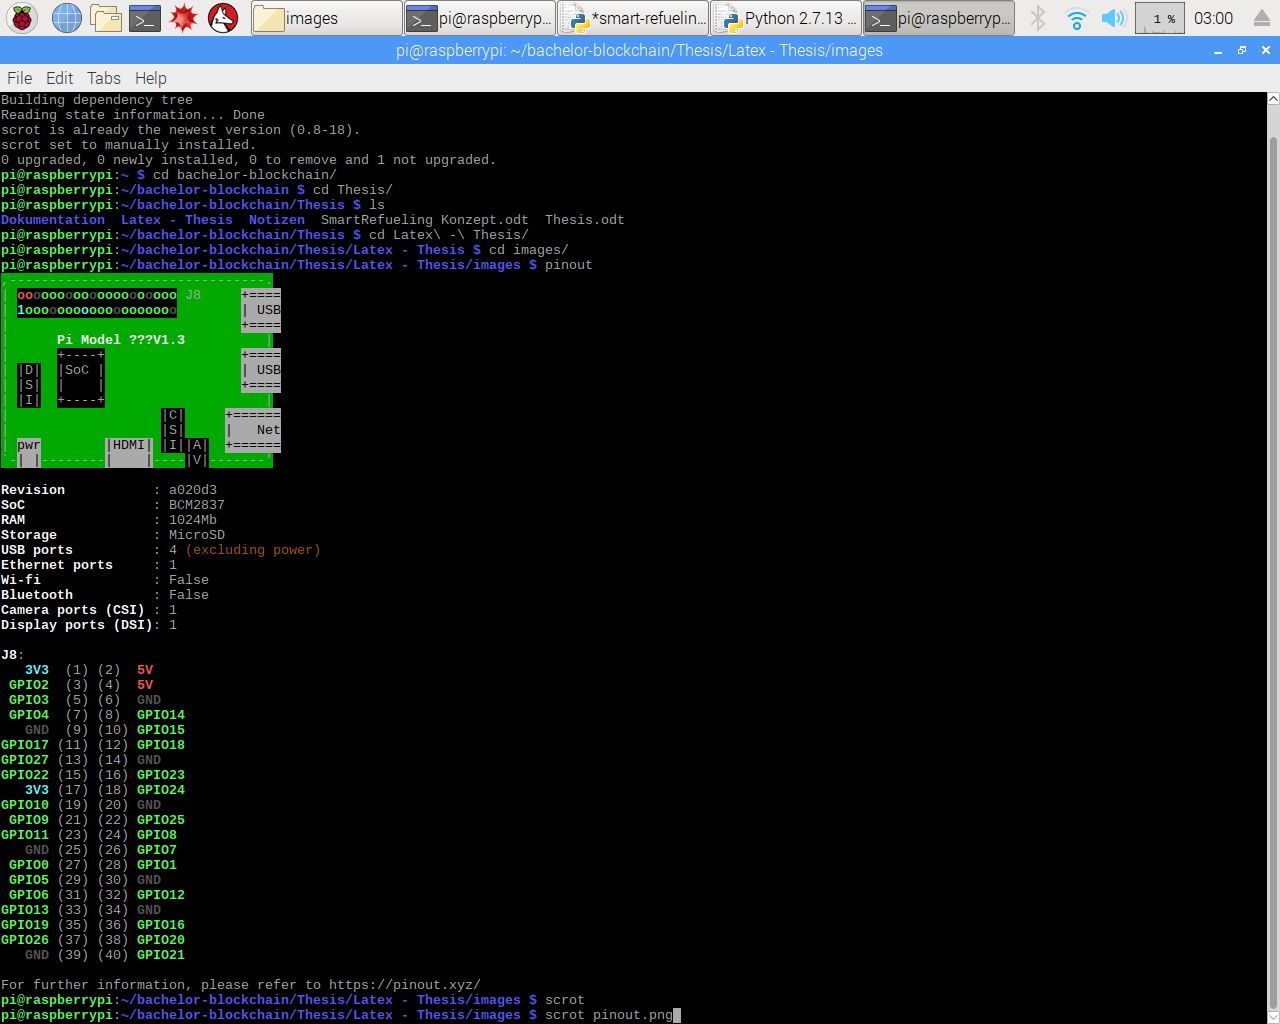
\includegraphics[scale=0.6]{pinout.png}%
\caption{Pinout-Ausgabe}
\end{figure}

Die Komponenten m�ssen in das Steckbrett gesteckt werden, sodass sie erreichbar bleiben, um sie zu verkabeln und zugleich nutzen zu k�nnen. F�r eine optimale �bersicht wurden die Komponenten mittig platziert.

F�r die Umsetzung m�ssen diese Komponenten f�r den Nutzer interagierbar sein, dazu werden sie mit zuf�lligen, freien GPIO-Pins verbunden.

\begin{table}[H]%
\centering
\begin{tabular}{l|l}
Komponente & GPIO-Pin\\
\hline
Button 1 & 11\\
Button 2 & 22\\
LED & 10
\end{tabular}
\caption{Korrespondenz der Buttons mit den GPIO-Pins}
\label{buttonlayout}
\end{table}

\subsubsection{PyOTA}
Bei PyOTA handelt es sich um eine Python-Bibliothek f�r IOTA. Sie implementiert die API und unterst�tzt Funktionalit�ten um eine Transaktion eigenst�ndig erstellen zu k�nnen\footnote{siehe dazu https://pyota.readthedocs.io/en/latest/}.

Um die Bibliothek f�r die Umsetzung zur Verf�gung zu stellen kann sie �ber das Paketverwaltungsprogramm f�r die Umgebung installiert werden.
\begin{lstlisting}[language=bash]
> pip install pyota
\end{lstlisting}

Eine wichtige Abh�ngigkeit (Dependancy) von PyOTA ist die Cryptography-Bibliothek. Diese wird nicht automatisch heruntergeladen und installiert, sondern dies muss manuell geschehen\footnote{mehr Informationen dazu https://cryptography.io/en/latest/installation/}.

Weiterhin muss angemerkt werden, das bei Raspbian kein System-Pfad zu den zus�tzlich installierten Paketen (per pip install) f�r Python2.7 gibt. Demzufolge muss der Pfad vor jedem Programmstart in das Suchverzeichnis hinzugef�gt werden. Dies geschieht mit folgendem Code:
\begin{lstlisting}[language=Python]
import sys
sys.path.append("/home/pi/.local/lib/python2.7/site-packages")  #path muss erweitert werden damit PyOta librarys gefunden werden k�nnen
\end{lstlisting}

\subsection{Ergebnis der Vorbereitung}
Nachdem alle Vorbedingungen erf�llt sind, ist der Raspberry Pi einsatzbereit um ein Programm zu erstellen und auszuf�hren, welches auf Benutzereingaben an Kn�pfen horcht, visuelles Feedback gibt und mit der PyOta-Bibliothek arbeitet.

\section{Umsetzung}
In diesem Abschnitt sollen die ausgew�hlten Programmierans�tze gezeigt und besprochen werden. Es soll ein �berblick �ber die verwendeten Methoden geschaffen werden. Bei mehreren m�glichen Methoden soll dar�ber hinaus deutlich werden, warum die entsprechende Methode gew�hlt wurde.

\subsection{GPIO-Pins}
Auf dem Raspberry Pi m�ssen die GPIO-Pins vorkonfiguriert werden um danach einzelne Pins als Inputs oder Outputs setzen zu k�nnen. Die Funktionalit�t wird der vorinstallierten RPi.GPIO-Bibliothek entnommen. Sie wird zur Abk�rzung fortan mit "`GPIO"' referenziert.
\begin{lstlisting}[language=Python]
import RPi.GPIO as GPIO     #importiere GPIO-Bibliothek f�r Ein-/Ausgaben von Inputs und Outputs (Buttons/LEDs)
\end{lstlisting}

Zum Ansprechen der Pins muss bestimmt werden, welche Pins mit welcher Nummer korrespondieren. Zum Beispiel hat Pin 12 eine Zweideutigkeit in dem Sinne, dass er zum einen Pin 12 bei einer, numerisch sortierten Aneinanderreihung, der zw�lfte Pin des Panels ist. Zum anderen kann sich Pin 12 auch auf den Namen des Pins beziehen, in diesem Beispiel "`GPIO12"', welcher sich nicht an einer numerischen Anordnung befindet.

Daher muss der Modus des Boards gesetzt werden mit folgender Code Zeile.
\begin{lstlisting}[language=Python]
GPIO.setmode(GPIO.BCM)
\end{lstlisting}
GPIO.BCM bezieht sich auf den Broadcom SOC (system on chip) Kanal, der angesprochen wird. Die Auswahl von dieser Variante hat keine Vor- oder Nachteile f�r das Projekt und wurde arbitr�r ausgew�hlt.

Nachdem der Modus eingestellt wurde kann nun die Datenrichtung der Pins bestimmt werden. Daf�r wird der Pin als Input oder als Output gesetzt.
\begin{lstlisting}[language=Python]
BUTTON1 = 11
BUTTON2 = 22
LED = 10

GPIO.setup(BUTTON1, GPIO.IN)
GPIO.setup(BUTTON2, GPIO.IN)
GPIO.setup(LED, GPIO.OUT, initial = False)
\end{lstlisting}

Nun sind die einzelnen Pins manipulierbar, bzw. auslesbar. Je nachdem ob man einen Output-Pin setzten m�chte oder einen Input-Pin auslesen m�chte, sind verschiedene Funktionen verwendbar.

Zum Auslesen ob ein Knopf gedr�ckt wurde bietet sich die folgende einfache Implementierung an. Das Programm wartet solange, bis der Knopf gedr�ckt und losgelassen wurde.
\begin{lstlisting}[language=Python]
def wait_for_button_click(button):
    while not GPIO.input(button):
        pass
    while GPIO.input(button):
        pass
\end{lstlisting}
Wobei der Parameter 'button' die Pin-Nummer referenziert.\\
Es bieten sich auch andere, effizientere Methoden an, jedoch ist diese Implementierung f�r den Prototypen ausreichend.

Um einen Output wie zum Beispiel die LED zu setzen, ben�tigen wir diese Code-Zeile:
\begin{lstlisting}[language=Python]
GPIO.output(LED, True)
\end{lstlisting}

\subsection{IOTA Einrichtung}
Unter der Einrichtung von IOTA ist zu verstehen, die IOTA-Bibliothek so zu utilisieren, dass mit der API eine Transaktion in das Tangle-Netzwerk ver�ffentlicht werden kann. F�r so eine Funktionalit�t bietet sich das Iota-Objekt an. Dieses wird dank des iota-Moduls bereitgestellt.
\begin{lstlisting}[language=Python]
from iota import Iota
\end{lstlisting}

Damit nun das Iota Objekt initialisiert werden kann, braucht es zwei Argumente. Den Seed, und eine Adresse zu einer Full-Node.

\paragraph{Seed} Der Seed "`DSPOAXMVSC99IUIVJXTIBZFATVFKTCLLJYOLAGSMFJGFXAWEB9GNTQWEDVRYHKIOQF9T9IZY9IVPKTSZK"' wurde aus einer zuf�lligen Kombination der Gro�buchstaben 'A-Z' und der Nummer 9 eigenh�ndig generiert und wird f�r den Prototypen genutzt. Im Programmcode ist der Seed hinterlegt, dies k�nnte bei einer realistischen Umgebung zu Sicherheitsrisiken f�hren, f�r die prototypische Umsetzung gen�gt es.

\paragraph{Full-Node} Aus einer Liste im Internet\footnote{siehe https://iotasalad.org/nodes}, in der einige Full-Nodes aufgelistet sind, wurde die folgende Adresse beliebig ausgesucht: https://potato.iotasalad.org:14265. Der Full-Node �bernimmt die Arbeit die erstellte Transaktion in das Tangle zu ver�ffentlichen, da der Raspberry Pi zu leistungsschwach ist um den Proof-Of-Work zeiteffizient zu �bernehmen.

Aus den gegebenen Parametern kann das Iota-Objekt erstellt werden.
\begin{lstlisting}[language=Python]
seed = "DSPOAXMVSC99IUIVJXTIBZFATVFKTCLLJYOLAGSMFJGFXAWEB9GNTQWEDVRYHKIOQF9T9IZY9IVPKTSZK"  
fullnode_url = "https://potato.iotasalad.org:14265"
api = Iota(fullnode_url, seed)
\end{lstlisting}

Es ist nun m�glich, grundlegende Funktionen wie Adressgenerierung nutzen zu k�nnen.

\subsection{IOTA Transaktion}
Um eine Transaktion zu erstellen werden f�r diese Implementierung die Klassen ProposedTransaction, ProposedBundle, Address, Tag und TryteString zus�tzlich zu Iota von dem iota-Modul genutzt.
\begin{lstlisting}[language=Python]
from iota import Iota, ProposedTransaction, ProposedBundle, Address, Tag, TryteString
\end{lstlisting}

Vorerst muss ein "`Vorabtransaktions"'-Objekt erstellt werden mit Adresse, Wert, Tag und Message.
\begin{lstlisting}[language=Python]
proposedTrx = ProposedTransaction(
    address = Address(reciever_address),
    value = 0,
    tag = Tag("BACHELORTEST"),
    message = TryteString.from_string("This is a test transaction")
)
proposedBundle = ProposedBundle([proposedTrx])
\end{lstlisting}
Das Transaktionsobjekt wird gef�llt mit der Empf�ngeradresse, dem Wert 0 (eine "`Meta Transaction"'), einem Tag welcher mithilfe des Tag-Objekts erstellt wird und einer beliebigen Nachricht, welche mithilfe von TryteString in Trits umgewandelt wird. Abschlie�end wird ein "`Vorabbundle"' erstellt, welches mit der Vorabtransaktion bef�llt wird.

Dieses Vorabbundle muss gepr�ft und signiert werden, daf�r wird es als Parameter an die vorher erstellte Iota-Instanz �bergeben. Der Aufruf gibt ein vorbereitetes Bundle zur�ck, welches mittels API-Aufruf an die Full-Node verschickt wird. Dort wird sie abschlie�end verarbeitet und in das Tangle-Netzwerk ver�ffentlicht.
\begin{lstlisting}[language=Python]
preparedBundle = api.prepare_transfer(proposedBundle)
publishedBundle = api.send_transfer(depth = 3, transfers = proposedBundle)
\end{lstlisting}

Die Hash des PublishedBundle-Objekts kann genutzt werden, um die Transaktion nachzuvollziehen\footnote{z.B auf https://iotasear.ch/}.

\subsection{Kommunikation mit Tankstelle}
Die Kommunikation mit der Tankstelle erfolgt �ber eine REST API. Dies ist vereinfacht betrachtet eine Schnittstelle auf die �ber HTTP zugegriffen werden kann. Hierf�r bietet sich das vorinstallierte requests-Modul an.
\begin{lstlisting}[language=Python]
import requests #importiere requests-Bibliothek um HTTP-Anfragen zu erstellen
\end{lstlisting}

Ein Beispiel eines Anwendungsfalles ist das Beenden des Tankvorgangs. Der Code hierf�r ist in einer Methode ausgelagert mit den Argumenten 'route' und 'carId'. Die 'route' ist die Schnittstelle die angesprochen werden soll, in diesem Beispiel "`endFueling"'. Die 'carId' ist eine von der Tankstelle zugewiesene Nummer. Das Beispiel verschickt eine Anfrage an den Server (die Tankstelle) mit einem Parameter, der Identifikationsnummer des Autos, und gibt die Antwort zur�ck.
\begin{lstlisting}[language=Python]
endFuelingData = call_api("endFueling", carId)

def call_api(route, carId):
		params = {
				"id": carId
		}
	response = requests.get(fueling_url + route, params)
return response.json()
\end{lstlisting}


\chapter{Ergebnis der Umsetzung}
Was aus den vorherigen Abschnitten folgt, ist ein Programm, welches mit einem Server �ber eine Rest-Schnittstelle kommunizieren kann und eigenst�ndig eine Transaktion ausf�hren kann. Mit dieser Applikation werden die Bezahlvorg�nge mit IOTAs abgewickelt.

Um das Ergebnis zu veranschaulichen wird das Programm vorgespielt.

...... Einmal probedurchlaufen mit dem Programm und erkl�ren wie das mit dem vorher erkl�rten zusammenh�ngt

Die API wird im ersten Schritt gestartet. Sollte die Verbindung zu der Datenbank gelingen erscheint die Nachricht, dass die API gestartet sei und auf den Port 1717 h�rt. (PICTURE start\_API)
\chapter{Fazit}
Abschlie�end werden die ausgearbeiteten Ergebnisse zusammengefasst und besprochen. Zudem wird ein Ausblick auf weitere Forschungsbereiche gegeben, die in dieser Arbeit nicht untersucht wurden.

\section{Zusammenfassung}
Der analytische Teil der Arbeit zeigt, dass eine Nutzung der Distributed Ledger Technologien in einer zuk�nftigen Umgebung durchaus denkbar ist. Wenn auch einige Bedenken seitens der Sicherheit gegeben sind. So ist es letztendlich schwer zu sagen ob die Einf�hrung der Quantencomputer nicht weitere Angriffsfl�chen auf die Kryptow�hrungen offenbaren als in dieser Ausarbeitung untersucht wurden sind. Denn die Sicherheit der kryptographischen Funktionen ist nur gegeben solange keine L�sungen f�r die zugrundeliegenden Probleme gefunden wurden.

Abseits der Verwendung als Kryptow�hrung k�nnen Distributed Ledger Technologien auch f�r die Datenspeicherung oder zum Versenden von Informationen genutzt werden. Diese experimentellen Implementierungen zeugen davon, dass das Potential noch nicht ausgesch�pft ist.

Zugleich best�tigt die prototypische Umsetzung der m�glichen Tankanwendung, dass eine Nutzung der Kryptow�hrungen f�r allt�gliche Prozesse schon gegenw�rtig m�glich ist. Da sich das Potential der Technologien nicht ausschlie�lich auf die Funktion als W�hrung beschr�nkt, ist mit weiteren Implementierungen im Bereich der Datenverarbeitung sowie Datensicherung zu rechnen.

Vorherzubestimmen welche Distributed Ledger Technologie sich behaupten k�nnte ist kaum Vorhersehbar. Jede Implementierung visiert unterschiedliche Ziele an und daher ist es wahrscheinlich, dass weiterhin eine Vielzahl an diversen Distributed Ledger Technologien existieren wird. Aufgrund der nicht ausgereiften Sicherheit ist jedoch �ber den momentanen Stand IOTAs keine endg�ltige Prognose aufzustellen.

\section{Ausblick}
Diese Arbeit hat sich mit der allgemeinen Technologie diverser Kryptow�hrungen besch�ftigt. Dies wurde in Aussicht auf die Beantwortung der Fragestellung durchgef�hrt, inwiefern Distributed Ledger Technologien zukunftstauglich sind. Dabei wurden einige weiterf�hrende Untersuchungen vernachl�ssigt, die im Folgenden kurz aufgef�hrt werden:

\subsection{Auswirkungen auf die Finanzwirtschaft}
Kryptow�hrungen sind Werteinheiten mit denen physische Gegenst�nde, sowohl im Internet als auch in einigen lokalen Gesch�ftstellen, erworben werden k�nnen. Bitcoin und IOTA verwenden pseudonymisierte Benutzerdaten, welche nicht den Besitzern direkt zugeordnet werden k�nnen. Aufgrund dieser Eigenschaft ist es deutlich erschwert den Geldfluss zu beobachten, zu regulieren oder zu unterbinden. Die Auswirkungen dieser Eigenschaften auf die zuk�nftige Finanzwirtschaft wurde in dieser Arbeit nicht behandelt.

\subsection{Die Funktion IOTAs neben der Kryptow�hrung}
IOTA bietet neben der Funktion als Kryptow�hrung noch weitere attraktive Funktionen. So ist es m�glich Dateien in Form eines JSON - Objektes an ein Ziel zu senden. Dabei ist es nicht von Belangen ob das Gegen�ber ein Mensch oder eine Maschine ist. Diese Eigenschaft, kombiniert mit der grenzenlosen Skalierbarkeit der Datenmenge k�nnte das momentane "`Client - Server"' Modell durch ein neues ersetzen. Auch die Art wie Daten im Internet publiziert und erreicht werden, k�nnte durch die Architektur des Tangle-Netzwerkes umgedacht werden.

\bibliographystyle{geralpha}
\bibliography{quellen}

\cleardoublepage
\pagestyle{plain}
\section*{Arbeitsteilung}
\pagenumbering{gobble}
Diese Seite stellt dar, welcher Autor ein bestimmtes Kapitel ausgearbeitet hat. In den wesentlichen Hauptkapiteln bestand eine klare Arbeitsteilung, in den anderen wurden beide Autoren f�r die Bearbeitung herangezogen.

Spatz, Janusz: \textbf{S}\\
Altrock, Jens: \textbf{A}\\

\begin{center}
\begin{tabular}{|l|c|}
\hline
Kapitel & Bearbeiter\\
\hline
1. Einleitung & A \& S\\
2. Grundlagen & \\
2.1 Hardware & S\\
2.2 Hash Tree (Merkle Tree) & A\\
2.3 Proof-of-Work (Hashcash) & A\\
2.4 Internet of Things (IoT) & S\\
2.5 Industrie 4.0 & S\\
2.6 Trits, Trytes \& Tryte-Alphabet & A\\
2.7 Distributed Ledger & A\\
2.8 Hash & A\\
2.9 Wallet & S\\
2.10 Restful API & A\\
2.11 Zusammenfassung & A \& S\\
3 Analyse der DLT & A \& S\\
4 Funktion & A\\
5 Sicherheit & S\\
6 Nutzen & A \& S\\
7 Ergebnis & A \& S\\
8 Realisierung des Prototypen & A \& S\\
9 Fahrzeug - Client & S\\
10 Tankstelle - Server & A\\
11 Ergebnis der Umsetzung & A \& S\\
12 Fazit & A \& S\\
\hline
\end{tabular}
\end{center}


\end{document}